\documentclass{article}
\usepackage[utf8]{inputenc}
\usepackage[margin=2cm]{geometry}

\usepackage{graphicx}
\usepackage{tikz}
\usepackage{enumitem}
\usepackage[nobreak]{mdframed} % The nobreak option should probably be set locally in the final document, since breaks may be required in longer theorems.

% custom header/footer
\usepackage{fancyhdr}
\pagestyle{fancy}
\renewcommand{\headrulewidth}{0pt}
\fancyhf{}
\rfoot{\textsf{\thepage}}
\lfoot{\textsf{Suzie Brown}}

%annotations
\usepackage{color}
\usepackage{xspace}
\newcommand{\seb}[1]{\xspace\textcolor{red}{#1}\xspace}

% bibliography
\usepackage[round, sort&compress]{natbib}
\usepackage{har2nat}
\bibliographystyle{agsm}

% maths
\usepackage{amsmath}
\usepackage{amssymb}
\usepackage{amsthm}
\usepackage[mathscr]{euscript}
\usepackage{bbm}
\newmdtheoremenv{theorem}{Theorem}
\newmdtheoremenv{lemma}{Lemma}
\newcommand{\Prob}{\mathbb{P}}
\newcommand{\E}{\mathbb{E}}
\newcommand{\Et}{\mathbb{E}_t}
\newcommand{\V}{\operatorname{Var}}
\newcommand{\I}[1]{\mathbbm{1}_{\{#1\}}}
\newcommand{\1}[1]{\mathbbm{1}_{#1}}
\newcommand{\Mn}{\operatorname{Multinomial}}
\renewcommand{\qedsymbol}{$\blacksquare$}

%\allowdisplaybreaks

\title{Weak convergence proof v.2 (neater) (in progress)}
\author{Suzie Brown}

\begin{document}
\maketitle
\thispagestyle{fancy}

\section*{Bounds on sum-products}

\begin{lemma}\label{thm:sumprod1}
Fix $t>0$, $l\in\mathbb{N}$.
\begin{equation}
t^l - \left( \sum_{s=1}^{\tau_N(t)} c_N(s)^2 \right) \binom{l}{2} (t+1)^{l-2} 
\leq \sum_{s_1\neq\dots\neq s_l}^{\tau_N(t)} \prod_{j=1}^l c_N(s_j)
\leq t^l + c_N(\tau_N(t)) (t+1)^l .
\end{equation}
\end{lemma}

\begin{proof}
As pointed out in \citet[Equation (8)]{koskela2018}, 
\begin{equation}\label{eq:002}
\sum_{s_1\neq\dots\neq s_l}^{\tau_N(t)} \prod_{j=1}^l c_N(s_j)
\geq \left( \sum_{s=0}^{\tau_N(t)} c_N(s) \right)^l
        - \binom{l}{2} \left( \sum_{s=0}^{\tau_N(t)} c_N(s)^2 \right)
        \left( \sum_{s=0}^{\tau_N(t)} c_N(s) \right)^{l-2} .
\end{equation}
By definition of $\tau_N$, 
\begin{equation}\label{eq:003}
t 
\leq \sum_{s=0}^{\tau_N(t)} c_N(s) 
\leq t+1 .
\end{equation}
Substituting these bounds into the RHS of \eqref{eq:002} yields the lower bound.

It is a true fact that
\begin{equation}\label{eq:005}
\sum_{s_1\neq\dots\neq s_l}^{\tau_N(t)} \prod_{j=1}^l c_N(s_j)
\leq \left( \sum_{s=0}^{\tau_N(t)} c_N(s) \right)^l ,
\end{equation}
as can be seen by considering the multinomial expansion of the RHS.
This is further bounded by
\begin{equation}
\left( \sum_{s=0}^{\tau_N(t)} c_N(s) \right)^l
\leq \left( \sum_{s=0}^{\tau_N(t) -1} c_N(s) + c_N(\tau_N(t)) \right)^l
\leq \left[ t + c_N(\tau_N(t)) \right]^l ,
\end{equation}
again using the definition of $\tau_N$.
A binomial expansion yields
\begin{equation}
\left[ t + c_N(\tau_N(t)) \right]^l
= t^l + \sum_{i=0}^{l-1} \binom{l}{i} t^i c_N(\tau_N(t))^{l-i}
= t^l + c_N(\tau_N(t)) \sum_{i=0}^{l-1} \binom{l}{i} t^i c_N(\tau_N(t))^{l-1-i} ,
\end{equation}
then since $c_N(s) \leq 1$ for all $s$,
\begin{equation}
\sum_{i=0}^{l-1} \binom{l}{i} t^i c_N(\tau_N(t))^{l-1-i}
\leq \sum_{i=0}^{l-1} \binom{l}{i} t^i
\leq (t+1)^l .
\end{equation}
Putting this together yields the upper bound.
\end{proof}


\begin{lemma}\label{thm:sumprod2}
Fix $t>0$, $l\in\mathbb{N}$.
Let $B$ be a positive constant which may depend on $n$.
\begin{equation}
\sum_{s_1\neq\dots\neq s_l}^{\tau_N(t)} \prod_{j=1}^l 
        \left[ c_N(s_j) + B D_N(s_j) \right]
\leq \sum_{s_1\neq\dots\neq s_l}^{\tau_N(t)} \prod_{j=1}^l c_N(s_j)
        + \left( \sum_{s=1}^{\tau_N(t)} D_N(s) \right) (t+1)^{l-1} (1+B)^l .
\end{equation}
\end{lemma}

\begin{proof}
We start with a binomial expansion:
\begin{align}
\sum_{s_1\neq\dots\neq s_l}^{\tau_N(t)} \prod_{j=1}^l 
        \left[ c_N(s_j) + B D_N(s_j) \right]
&= \sum_{s_1\neq\dots\neq s_l}^{\tau_N(t)} \sum_{\mathcal{I} \subseteq [l]}
        B^{l-|\mathcal{I}|} \left( \prod_{i\in\mathcal{I}} c_N(s_i) \right)
        \left( \prod_{j\notin\mathcal{I}} D_N(s_j) \right) \notag\\
&= \sum_{\mathcal{I} \subseteq [l]} B^{l-|\mathcal{I}|}
        \sum_{s_1\neq\dots\neq s_l}^{\tau_N(t)}
        \left( \prod_{i\in\mathcal{I}} c_N(s_i) \right)
        \left( \prod_{j\notin\mathcal{I}} D_N(s_j) \right) \label{eq:010}
\end{align}
where $[l] := \{1,\dots,l\}$. Since the sum is over all permutations of $r_1,\dots,r_l$, we may arbitrarily choose an ordering for $\{1,\dots,l\}$ such that $\mathcal{I} = \{ 1,\dots, |\mathcal{I}| \}$:
\begin{equation}
\sum_{\mathcal{I} \subseteq [l]} B^{l-|\mathcal{I}|}
        \sum_{s_1\neq\dots\neq s_l}^{\tau_N(t)}
        \left( \prod_{i\in\mathcal{I}} c_N(s_i) \right)
        \left( \prod_{j\notin\mathcal{I}} D_N(s_j) \right)
= \sum_{I=0}^l \binom{l}{I} B^{l-I} \sum_{s_1\neq\dots\neq s_l}^{\tau_N(t)}
        \left( \prod_{i=1}^I c_N(s_i) \right)
        \left( \prod_{j=I+1}^l D_N(s_j) \right) .
\end{equation}
Separating the term $I=l$,
\begin{align}
\sum_{I=0}^l \binom{l}{I} B^{l-I} \sum_{s_1\neq\dots\neq s_l}^{\tau_N(t)}
        \left( \prod_{i=1}^I c_N(s_i) \right)
        &\left( \prod_{j=I+1}^l D_N(s_j) \right)
= \sum_{s_1\neq\dots\neq s_l}^{\tau_N(t)} \prod_{j=1}^l c_N(s_j) \notag\\
&\qquad+ \sum_{I=0}^{l-1} \binom{l}{I} B^{l-I} 
        \sum_{s_1\neq\dots\neq s_l}^{\tau_N(t)}
        \left( \prod_{i=1}^I c_N(s_i) \right) \left( \prod_{j=I+1}^l D_N(s_j) \right). \label{eq:012}
\end{align}
In the second line, there is always at least one $D_N$ term, and $c_N(s) \leq D_N(s)$ for all $s$, so we can write
\begin{align}
\sum_{I=0}^{l-1}\binom{l}{I} B^{l-I} \sum_{s_1\neq\dots\neq s_l}^{\tau_N(t)}
        \left( \prod_{i=1}^I c_N(s_i) \right) \left( \prod_{j=I+1}^l D_N(s_j) \right)
&\leq \sum_{I=0}^{l-1}\binom{l}{I} B^{l-I} 
        \sum_{s_1\neq\dots\neq s_l}^{\tau_N(t)}
        \left( \prod_{i=1}^{l-1} c_N(s_i) \right) D_N(s_l) \notag\\
&\leq \sum_{I=0}^{l-1}\binom{l}{I} B^{l-I} 
        \left( \sum_{s_1\neq\dots\neq s_{l-1}}^{\tau_N(t)} 
        \prod_{i=1}^{l-1} c_N(s_i) \right) 
        \sum_{s_l=1}^{\tau_N(t)} D_N(s_l) \notag\\
&\leq \sum_{I=0}^{l-1}\binom{l}{I} B^{l-I} (t+1)^{l-1}
        \sum_{s=1}^{\tau_N(t)} D_N(s) \label{eq:013}
\end{align}
using \eqref{eq:005} and \eqref{eq:003}.
Finally, by the Binomial Theorem,
\begin{equation}\label{eq:014}
\sum_{I=0}^{l-1}\binom{l}{I} B^{l-I} (t+1)^{l-1}
        \sum_{s=1}^{\tau_N(t)} D_N(s)
\leq \left( \sum_{s=1}^{\tau_N(t)} D_N(s) \right) (t+1)^{l-1} (1+B)^l ,
\end{equation}
which, together with \eqref{eq:012}, concludes the proof.
\end{proof}


\begin{lemma}\label{thm:sumprod3}
Fix $t>0$, $l\in\mathbb{N}$.
Let $B$ be a positive constant which may depend on $n$.
\begin{equation}
\sum_{s_1\neq\dots\neq s_l}^{\tau_N(t)} \prod_{j=1}^l 
        \left[ c_N(s_j) - B D_N(s_j) \right]
\geq \sum_{s_1\neq\dots\neq s_l}^{\tau_N(t)} \prod_{j=1}^l c_N(s_j)
        - \left( \sum_{s=1}^{\tau_N(t)} D_N(s) \right) (t+1)^{l-1} (1+B)^l .
\end{equation}
\end{lemma}

\begin{proof}
A binomial expansion and subsequent manipulation as in \eqref{eq:010}--\eqref{eq:012} gives
\begin{align}
\sum_{s_1\neq\dots\neq s_l}^{\tau_N(t)} \prod_{j=1}^l 
        \left[ c_N(s_j) - B D_N(s_j) \right]
&= \sum_{\mathcal{I} \subseteq [l]} (-B)^{l-|\mathcal{I}|}
        \sum_{s_1\neq\dots\neq s_l}^{\tau_N(t)}
        \left( \prod_{i\in\mathcal{I}} c_N(s_i) \right)
        \left( \prod_{j\notin\mathcal{I}} D_N(s_j) \right) \notag\\
&= \sum_{I=0}^l \binom{l}{I} (-B)^{l-I} 
        \sum_{s_1\neq\dots\neq s_l}^{\tau_N(t)}
        \left( \prod_{i=1}^I c_N(s_i) \right)
        \left( \prod_{j=I+1}^l D_N(s_j) \right) \notag\\
&= \sum_{s_1\neq\dots\neq s_l}^{\tau_N(t)} \prod_{j=1}^l c_N(s_j)
        + \sum_{I=0}^{l-1} \binom{l}{I} (-B)^{l-I} 
        \sum_{s_1\neq\dots\neq s_l}^{\tau_N(t)}
        \left( \prod_{i=1}^I c_N(s_i) \right) 
        \left( \prod_{j=I+1}^l D_N(s_j) \right) \notag\\
&\geq \sum_{s_1\neq\dots\neq s_l}^{\tau_N(t)} \prod_{j=1}^l c_N(s_j)
        - \sum_{I=0}^{l-1} \binom{l}{I} B^{l-I} 
        \sum_{s_1\neq\dots\neq s_l}^{\tau_N(t)}
        \left( \prod_{i=1}^I c_N(s_i) \right) \left( \prod_{j=I+1}^l D_N(s_j) \right)
\end{align}
where the last inequality just multiplies some positive terms by $-1$.
Then \eqref{eq:013}--\eqref{eq:014} can be applied directly (noting that an upper bound on negative terms gives a lower bound overall):
\begin{equation}
- \sum_{I=0}^{l-1} \binom{l}{I} B^{l-I} 
        \sum_{s_1\neq\dots\neq s_l}^{\tau_N(t)}
        \left( \prod_{i=1}^I c_N(s_i) \right) \left( \prod_{j=I+1}^l D_N(s_j) \right)
\geq \left( \sum_{s=1}^{\tau_N(t)} D_N(s) \right) (t+1)^{l-1} (1+B)^l 
\end{equation}
which concludes the proof.
\end{proof}


\section*{Main components of weak convergence}

\begin{lemma}[Basis step]\label{thm:basis}
For any $0 < t < \infty$,
\begin{equation}
\lim_{N\to\infty} \E\left[ \prod_{r=1}^{\tau_N(t)} (1-p_r) \right] 
= e^{-\alpha_n t}
\end{equation}
where $\alpha_n := n(n-1)/2$.
\end{lemma}

\begin{proof}
We start by showing that
$\lim_{N\to\infty}\E\left[ \prod_{r=1}^{\tau_N(t)} (1-p_r) \right] 
\leq e^{-\alpha_n t}$.\\
From \citet[Lemma 1 Case 1]{koskela2018}, taking $\xi=\Delta$, we have for each $r$
\begin{equation} \label{eq:018}
1-p_r
= p_{\Delta\Delta}(r) \leq 1 - \alpha_n (1+O(N^{-1})) 
        \left[ c_N(r) - B_n^\prime D_N(r) \right] 
\end{equation}
where the $O(N^{-1})$ term does not depend on $r$.
Applying a multinomial expansion and then separating the positive and negative terms,
\begin{align}
\prod_{r=1}^{\tau_N(t)} (1-p_r)
&\leq 1 + \sum_{l=1}^{\tau_N(t)} (- \alpha_n)^l (1+O(N^{-1})) 
        \frac{1}{l!} \sum_{s_1\neq\dots\neq s_l}^{\tau_N(t)}\prod_{j=1}^l
        \left[ c_N(s_j) - B_n^\prime D_N(s_j) \right] \notag\\
&= 1 + \sum_{\substack{l=2 \\ \text{even} }}^{\tau_N(t)} 
        \alpha_n^l (1+O(N^{-1})) \frac{1}{l!} 
        \sum_{s_1\neq\dots\neq s_l}^{\tau_N(t)}\prod_{j=1}^l
        \left[ c_N(s_j) - B_n^\prime D_N(s_j) \right] \notag\\
    &\qquad- \sum_{\substack{l=1 \\ \text{odd} }}^{\tau_N(t)} 
        \alpha_n^l (1+O(N^{-1})) \frac{1}{l!} 
        \sum_{s_1\neq\dots\neq s_l}^{\tau_N(t)}\prod_{j=1}^l
        \left[ c_N(s_j) - B_n^\prime D_N(s_j) \right] . \label{eq:019}
\end{align}
This is further bounded by applying Lemma~\ref{thm:sumprod3} and then both bounds of Lemma~\ref{thm:sumprod1}:
\begin{align}
\prod_{r=1}^{\tau_N(t)} (1-p_r)
&\leq 1 + \sum_{\substack{l=2 \\ \text{even} }}^{\tau_N(t)} 
        \alpha_n^l (1+O(N^{-1})) \frac{1}{l!} 
        \sum_{s_1\neq\dots\neq s_l}^{\tau_N(t)}\prod_{j=1}^l c_N(s_j) \notag\\
    &\qquad- \sum_{\substack{l=1 \\ \text{odd} }}^{\tau_N(t)} 
        \alpha_n^l (1+O(N^{-1})) \frac{1}{l!} 
        \left\{ \sum_{s_1\neq\dots\neq s_l}^{\tau_N(t)}\prod_{j=1}^l c_N(s_j)
        - \left( \sum_{s=1}^{\tau_N(t)} D_N(s) \right) 
        (t+1)^{l-1} (1+B_n^\prime)^l \right\} \notag\\
&\leq 1 + \sum_{\substack{l=2 \\ \text{even} }}^{\tau_N(t)} 
        \alpha_n^l (1+O(N^{-1})) \frac{1}{l!} 
        \left\{ t^l + c_N(\tau_N(t)) (t+1)^l \right\} \notag\\
    &\qquad- \sum_{\substack{l=1 \\ \text{odd} }}^{\tau_N(t)} 
        \alpha_n^l (1+O(N^{-1})) \frac{1}{l!} 
        \left\{ t^l - \left( \sum_{s=1}^{\tau_N(t)} c_N(s)^2 \right) 
        \binom{l}{2} (t+1)^{l-2}
        - \left( \sum_{s=1}^{\tau_N(t)} D_N(s) \right) 
        (t+1)^{l-1} (1+B_n^\prime)^l \right\} .
\end{align}
Collecting some terms,
\begin{align}
\prod_{r=1}^{\tau_N(t)} (1-p_r)
&\leq \sum_{l=0}^{\tau_N(t)} (-\alpha_n)^l (1+O(N^{-1})) \frac{1}{l!} t^l
        + c_N(\tau_N(t)) \sum_{\substack{l=2 \\ \text{even} }}^{\tau_N(t)}
        \alpha_n^l (1+O(N^{-1})) \frac{1}{l!} (t+1)^l \notag\\
    &\qquad+ \left( \sum_{s=1}^{\tau_N(t)} c_N(s)^2 \right)
        \sum_{\substack{l=1 \\ \text{odd} }}^{\tau_N(t)} \alpha_n^l
        (1+O(N^{-1})) \frac{1}{l!} \binom{l}{2} (t+1)^{l-2} \notag\\
    &\qquad+ \left( \sum_{s=1}^{\tau_N(t)} D_N(s) \right) 
        \sum_{\substack{l=1 \\ \text{odd} }}^{\tau_N(t)} \alpha_n^l
        (1+O(N^{-1})) \frac{1}{l!} (t+1)^{l-1} (1+B_n^\prime)^l \notag\\
&\leq \sum_{l=0}^{\infty} (-\alpha_n)^l (1+O(N^{-1})) \frac{1}{l!} t^l
        \I{\tau_N(t) \geq l}
        + c_N(\tau_N(t)) \exp[ \alpha_n (1+O(N^{-1})) (t+1) ] \notag\\
    &\qquad+ \left( \sum_{s=1}^{\tau_N(t)} c_N(s)^2 \right)
        \frac{1}{2} \alpha_n^2 \exp[ \alpha_n (1+O(N^{-1})) (t+1) ] \notag\\
    &\qquad+ \left( \sum_{s=1}^{\tau_N(t)} D_N(s) \right)
        \exp[ \alpha_n (1+O(N^{-1})) (t+1) (1+B_n^\prime) ] . \label{eq:021}
\end{align}
Now, taking the expectation and limit, then applying \citet[Equations (3.3)--(3.5)]{brown2021} and Lemma~\ref{thm:indicators_tau},
\begin{align}
\lim_{N\to\infty} \E \left[ \prod_{r=1}^{\tau_N(t)} (1-p_r) \right]
&\leq \sum_{l=0}^{\infty} (-\alpha_n)^l \frac{1}{l!} t^l
        \lim_{N\to\infty} \Prob \left[ \tau_N(t) \geq l \right]
    + \lim_{N\to\infty} \E \left[ c_N(\tau_N(t)) \right]
        \exp[ \alpha_n (t+1) ] \notag\\
    &\qquad+ \lim_{N\to\infty} \E \left[ \sum_{s=1}^{\tau_N(t)} 
        c_N(s)^2 \right]
        \frac{1}{2} \alpha_n^2 \exp[ \alpha_n (t+1) ] \notag\\
    &\qquad+ \lim_{N\to\infty} \E \left[ \sum_{s=1}^{\tau_N(t)} D_N(s) \right]
        \exp[ \alpha_n (t+1) (1+B_n^\prime) ] \notag\\
&= \sum_{l=0}^{\infty} (-\alpha_n)^l \frac{1}{l!} t^l
= e^{-\alpha_n t}. \label{eq:022}
\end{align}

It remains to show the corresponding lower bound
$\lim_{N\to\infty}\E\left[ \prod_{r=1}^{\tau_N(t)} (1-p_r) \right] 
\geq e^{-\alpha_n t}$.\\
From \citet[Equation (3.14)]{brown2021}, taking $\xi=\Delta$, we have
\begin{equation}\label{eq:023}
1-p_t 
= p_{\Delta\Delta}(t) \geq 1 - \alpha_n (1+O(N^{-1})) 
        \left[c_N(t) + B_n D_N(t) \right]
\end{equation}
where $B_n >0$ and the $O(N^{-1})$ term does not depend on $t$.
In particular,
\begin{equation}
1-p_t
= p_{\Delta\Delta}(t) \geq 1 - \frac{N^{n-2}}{(N-2)_{n-2}} \alpha_n c_N(t) 
        - \frac{N^{n-3}}{(N-3)_{n-3}} \alpha_n B_n D_N(t) .
\end{equation}
Since $D_N(s) \leq c_N(s)$ for all $s$ \citep[p.9]{koskela2018}, a sufficient condition for this bound to be non-negative is
\begin{equation}\label{eq:025}
E_r 
:= \left\{ c_N(r) \leq \frac{(N-3)_{n-3}}{N^{n-3}} 
        \frac{1}{\alpha_n} \left( \frac{N}{N-2} + B_n \right)^{-1} \right\} ,
\end{equation}
and we define $E := \bigcap_{r=1}^{\tau_N(t)} E_r$.
We now apply a multinomial expansion to the product, and split into positive and negative terms:
\begin{align}
\prod_{r=1}^{\tau_N(t)} (1-p_r)
&\geq \left\{ 1 + \sum_{l=1}^{\tau_N(t)} (-\alpha_n)^l (1+O(N^{-1})) 
        \frac{1}{l!} \sum_{s_1\neq\dots\neq s_l}^{\tau_N(t)}\prod_{j=1}^l
        \left[ c_N(s_j) + B_n D_N(s_j) \right] \right\} \1{E} \notag\\
&= \Bigg\{ 1 + \sum_{\substack{l=2 \\ \text{even} }}^{\tau_N(t)} 
        \alpha_n^l (1+O(N^{-1})) \frac{1}{l!} 
        \sum_{s_1\neq\dots\neq s_l}^{\tau_N(t)}\prod_{j=1}^l
        \left[ c_N(s_j) + B_n D_N(s_j) \right] \notag\\
    &\qquad- \sum_{\substack{l=1 \\ \text{odd} }}^{\tau_N(t)} 
        \alpha_n^l (1+O(N^{-1})) \frac{1}{l!}
        \sum_{s_1\neq\dots\neq s_l}^{\tau_N(t)}\prod_{j=1}^l
        \left[ c_N(s_j) + B_n D_N(s_j) \right] \Bigg\} \1{E}
\end{align}
This is further bounded by applying Lemma~\ref{thm:sumprod2} and both bounds in Lemma~\ref{thm:sumprod1}:
\begin{align}
\prod_{r=1}^{\tau_N(t)} (1-p_r)
&\geq \Bigg\{ 1 + \sum_{\substack{l=2 \\ \text{even} }}^{\tau_N(t)} 
        \alpha_n^l (1+O(N^{-1})) \frac{1}{l!} 
        \sum_{s_1\neq\dots\neq s_l}^{\tau_N(t)}\prod_{j=1}^l c_N(s_j) \notag\\
    &\qquad- \sum_{\substack{l=1 \\ \text{odd} }}^{\tau_N(t)} 
        \alpha_n^l (1+O(N^{-1})) \frac{1}{l!}
        \left[ \sum_{s_1\neq\dots\neq s_l}^{\tau_N(t)}\prod_{j=1}^l c_N(s_j)
        + \left( \sum_{s=1}^{\tau_N(t)} D_N(s) \right)
        (t+1)^{l-1} (1+B_n)^l \right] \Bigg\} \1{E} \notag\\
&\geq \Bigg\{ 1 + \sum_{\substack{l=2 \\ \text{even} }}^{\tau_N(t)} 
        \alpha_n^l (1+O(N^{-1})) \frac{1}{l!} 
        \left[ t^l - \left( \sum_{s=1}^{\tau_N(t)} c_N(s)^2 \right)
        \binom{l}{2}(t+1)^{l-2} \right] \notag\\
    &\qquad- \sum_{\substack{l=1 \\ \text{odd} }}^{\tau_N(t)} 
        \alpha_n^l (1+O(N^{-1})) \frac{1}{l!}
        \left[ t^l + c_N(\tau_N(t)) (t+1)^l
        + \left( \sum_{s=1}^{\tau_N(t)} D_N(s) \right)
        (t+1)^{l-1} (1+B_n)^l \right] \Bigg\} \1{E} .
\end{align}
Collecting terms,
\begin{align}
\prod_{r=1}^{\tau_N(t)} (1-p_r)
&\geq \sum_{l=0}^{\tau_N(t)} (-\alpha_n)^l (1+O(N^{-1})) 
        \frac{1}{l!} t^l \1{E}
        - \left( \sum_{s=1}^{\tau_N(t)} c_N(s)^2 \right)
        \sum_{\substack{l=2 \\ \text{even} }}^{\tau_N(t)} 
        \alpha_n^l (1+O(N^{-1})) \frac{1}{l!} \binom{l}{2}(t+1)^{l-2} \notag\\
    &\qquad- c_N(\tau_N(t)) \sum_{\substack{l=1 \\ \text{odd} }}^{\tau_N(t)} 
        \alpha_n^l (1+O(N^{-1})) \frac{1}{l!} (t+1)^l \notag\\
    &\qquad- \left( \sum_{s=1}^{\tau_N(t)} D_N(s) \right)
        \sum_{\substack{l=1 \\ \text{odd} }}^{\tau_N(t)} 
        \alpha_n^l (1+O(N^{-1})) \frac{1}{l!} (t+1)^{l-1} (1+B_n)^l \notag\\
&\geq \sum_{l=0}^{\infty} (-\alpha_n)^l (1+O(N^{-1})) 
        \frac{1}{l!} t^l \1{E} \I{ \tau_N(t) \geq l}
        - \left( \sum_{s=1}^{\tau_N(t)} c_N(s)^2 \right)
        \frac{1}{2} \alpha_n^2 \exp[ \alpha_n (1+O(N^{-1})) (t+1) ]\notag\\
    &\qquad- c_N(\tau_N(t)) \exp[ \alpha_n (1+O(N^{-1})) (t+1) ] \notag\\
    &\qquad- \left( \sum_{s=1}^{\tau_N(t)} D_N(s) \right)
        \exp[ \alpha_n (1+O(N^{-1})) (t+1) (1+B_n) ]. \label{eq:028}
\end{align}
Now, taking the expectation and limit, and applying \citet[Equations (3.3)--(3.5)]{brown2021} to show that all but the first sum vanish, and Lemmata \ref{thm:indicators_tau} and \ref{thm:indicators_cN} to show that $\lim_{N\to\infty} \Prob[ \{\tau_N(t) \geq l\} \cap E ] =1$,
\begin{align}
\lim_{N\to\infty} \E \left[ \prod_{r=1}^{\tau_N(t)} (1-p_r) \right]
&\geq \sum_{l=0}^{\infty} (-\alpha_n)^l (1+O(N^{-1})) \frac{1}{l!} t^l 
        \lim_{N\to\infty} \Prob\left[ \{\tau_N(t) \geq l\} \cap E \right] \notag\\
    &\qquad- \lim_{N\to\infty} \E \left[ \sum_{s=1}^{\tau_N(t)} c_N(s)^2 \right]
        \frac{1}{2} \alpha_n^2 \exp[ \alpha_n (t+1) ]\notag\\
    &\qquad- \lim_{N\to\infty} \E \left[ c_N(\tau_N(t)) \right] 
        \exp[ \alpha_n (t+1) ] \notag\\
    &\qquad- \lim_{N\to\infty} \E \left[ \sum_{s=1}^{\tau_N(t)} D_N(s) \right]
        \exp[ \alpha_n (t+1) (1+B_n) ] \notag\\
&= \sum_{l=0}^{\infty} (-\alpha_n)^l \frac{1}{l!} t^l
= e^{-\alpha_n t}. \label{eq:029}
\end{align}
Combining the upper and lower bounds in \eqref{eq:022} and \eqref{eq:029} respectively concludes the proof.
\end{proof}


\begin{lemma}[Induction step upper bound]\label{thm:inductionUB}
Fix $k \in \mathbb{N}$, $i_0:=0$, $i_k:=k$. For any sequence of times
$0 = t_0 \leq t_1 \leq \cdots \leq t_k \leq t$,
\begin{equation}\label{eq:030}
\lim_{N\to\infty} \E \left[ 
        \sum_{\substack{r_1 <\dots< r_k :\\ r_i \leq \tau_N(t_i) \forall i}}
        \left( \prod_{i=1}^k p_{r_i} \right)
        \left( \prod_{\substack{r=1 \\ \notin \{r_1,\dots,r_k\} }}^{\tau_N(t)} 
        (1-p_r) \right) \right]
\leq \alpha_n^k \sum_{l=0}^\infty \frac{1}{l!} (-\alpha_n)^l t^l 
        \sum_{\substack{i_1\leq \dots\leq i_{k-1}\\ \in \{0,\dots,k\} :
        \\ i_j \geq j \forall j}} 
        \prod_{j=1}^k \frac{(t_j - t_{j-1})^{i_j - i_{j-1}}}{(i_j - i_{j-1})! } .
\end{equation}
\end{lemma}

\begin{proof}
We use the bound on $(1-p_r)$ from \eqref{eq:018} and apply a multinomial expansion:
\begin{align}
\prod_{\substack{r=1 \\ \notin \{r_1,\dots,r_k\} }}^{\tau_N(t)} (1-p_r)
&\leq \prod_{\substack{r=1 \\ \notin \{r_1,\dots,r_k\} }}^{\tau_N(t)} 
        \left\{ 1 - \alpha_n  (1+O(N^{-1})) [ c_N(r) - B_n^\prime D_N(r) ] 
        \right\} \notag\\
&= 1 + \sum_{l=1}^{\tau_N(t) -k}
        (-\alpha_n)^l (1+O(N^{-1})) \frac{1}{l!}
        \sum_{\substack{s_1\neq\dots\neq s_l \\ \notin \{r_1,\dots,r_k\} }}
        ^{\tau_N(t)}
        \prod_{j=1}^l [ c_N(s_j) - B_n^\prime D_N(s_j) ] \notag\\
&= 1 + \sum_{l=1}^{\tau_N(t) -k}
        (-\alpha_n)^l (1+O(N^{-1})) \frac{1}{l!}
        \sum_{\substack{s_1\neq\dots\neq s_l }}^{\tau_N(t)}
        \prod_{j=1}^l [ c_N(s_j) - B_n^\prime D_N(s_j) ] \notag\\
    &\qquad- \sum_{l=1}^{\tau_N(t) -k}
        (-\alpha_n)^l (1+O(N^{-1})) \frac{1}{l!}
        \sum_{\substack{s_1\neq\dots\neq s_l \\ \exists i,i^\prime 
        : s_i=r_{i^\prime} }}
        \prod_{j=1}^l [ c_N(s_j) - B_n^\prime D_N(s_j) ] . \label{eq:031}
\end{align}
The penultimate line above is exactly the expansion we had in the basis step \eqref{eq:019}, except for the limit on $l$, and as such following the same arguments gives a bound like that in \eqref{eq:021}:
\begin{align}
1 + \sum_{l=1}^{\tau_N(t) -k}
        (-\alpha_n)^l (1+O(N^{-1})) \frac{1}{l!}
        &\sum_{\substack{s_1\neq\dots\neq s_l }}^{\tau_N(t)}
        \prod_{j=1}^l [ c_N(s_j) - B_n^\prime D_N(s_j) ] \notag\\
&\leq \sum_{l=0}^{\tau_N(t) -k} (-\alpha_n)^l (1+O(N^{-1})) \frac{1}{l!} t^l
    + c_N(\tau_N(t)) \exp[ \alpha_n (1+O(N^{-1})) (t+1) ] \notag\\
    &\qquad+ \left( \sum_{s=1}^{\tau_N(t)} c_N(s)^2 \right)
        \frac{1}{2} \alpha_n^2 \exp[ \alpha_n (1+O(N^{-1})) (t+1) ] \notag\\
    &\qquad+ \left( \sum_{s=1}^{\tau_N(t)} D_N(s) \right)
        \exp[ \alpha_n (1+O(N^{-1})) (t+1) (1+B_n^\prime) ] .
\end{align}
For the last line of \eqref{eq:031},
\begin{align}
- \sum_{l=1}^{\tau_N(t) -k} (-\alpha_n)^l (1+O(N^{-1})) \frac{1}{l!}
        &\sum_{\substack{s_1\neq\dots\neq s_l \\ \exists i,i^\prime 
        : s_i=r_{i^\prime} }}
        \prod_{j=1}^l \{ c_N(s_j) - B_n^\prime D_N(s_j) \} \notag\\
&\leq \sum_{l=1}^{\tau_N(t) -k} \alpha_n^l (1+O(N^{-1})) \frac{1}{l!}
        \sum_{\substack{s_1\neq\dots\neq s_l \\ \exists i,i^\prime 
        : s_i=r_{i^\prime} }}
        \prod_{j=1}^l \{ c_N(s_j) + B_n^\prime D_N(s_j) \} \notag\\
&\leq \sum_{l=1}^{\tau_N(t) -k} \alpha_n^l (1+O(N^{-1})) \frac{1}{l!}
        \sum_{\substack{s_1\neq\dots\neq s_l \\ \exists i,i^\prime 
        : s_i=r_{i^\prime} }}
        (1 + B_n^\prime)^l \prod_{j=1}^l c_N(s_j) \notag\\
&\leq \sum_{l=1}^{\tau_N(t) -k} \alpha_n^l (1+O(N^{-1}))
        \frac{1}{(l-1)!} \sum_{s_1 \in \{r_1,\dots,r_k\} } 
        \sum_{s_2\neq \dots\neq s_l}^{\tau_N(t)}
        (1 + B_n^\prime)^l \prod_{j=1}^l c_N(s_j) \notag\\
&= \sum_{s \in \{r_1,\dots,r_k\} } c_N(s)
        \sum_{l=1}^{\tau_N(t) -k} \alpha_n^l (1+O(N^{-1}))
        \frac{1}{(l-1)!}  (1 + B_n^\prime)^l
        \sum_{s_1\neq \dots\neq s_{l-1}}^{\tau_N(t)} 
        \prod_{j=1}^{l-1} c_N(s_j) \notag\\
&\leq \sum_{j=1}^k c_N(r_j)
        \sum_{l=1}^{\tau_N(t) -k} \alpha_n^l (1+O(N^{-1}))
        \frac{1}{(l-1)!}  (1 + B_n^\prime)^l (t+1)^{l-1} \notag\\
&\leq \left( \sum_{j=1}^k c_N(r_j) \right)
        \alpha_n (1 + B_n^\prime) 
        \exp[ \alpha_n (1+O(N^{-1})) (1 + B_n^\prime) (t+1) ] .
\end{align}
Putting these together, we have
\begin{align}
\prod_{\substack{r=1 \\ \notin \{r_1,\dots,r_k\} }}^{\tau_N(t)} (1-p_r)
&\leq \sum_{l=0}^{\tau_N(t) -k} (-\alpha_n)^l (1+O(N^{-1})) \frac{1}{l!} t^l
    + c_N(\tau_N(t)) \exp[ \alpha_n (1+O(N^{-1})) (t+1) ] \notag\\
    &\qquad+ \left( \sum_{s=1}^{\tau_N(t)} c_N(s)^2 \right)
        \frac{1}{2} \alpha_n^2 \exp[ \alpha_n (1+O(N^{-1})) (t+1) ] \notag\\
    &\qquad+ \left( \sum_{s=1}^{\tau_N(t)} D_N(s) \right)
        \exp[ \alpha_n (1+O(N^{-1})) (t+1) (1+B_n^\prime) ] \notag\\
    &\qquad+ \left( \sum_{j=1}^k c_N(r_j) \right)
        \alpha_n (1 + B_n^\prime)
        \exp[ \alpha_n (1+O(N^{-1})) (1 + B_n^\prime) (t+1) ] . \label{eq:034b}
\end{align}
Meanwhile, using the bound on $p_r$ from \eqref{eq:023} then applying a modification of Lemma~\ref{thm:sumprod2},
\begin{align}
\sum_{\substack{r_1 <\dots< r_k :\\ r_i \leq \tau_N(t_i) \forall i}}
        \prod_{i=1}^k p_{r_i}
&\leq \alpha_n^k (1+O(N^{-1})) 
        \sum_{\substack{r_1 <\dots< r_k :\\ r_i \leq \tau_N(t_i) \forall i}}
        \prod_{i=1}^k \left[ c_N(r_i) + B_n D_N(r_i) \right] \notag\\
&\leq \alpha_n^k (1+O(N^{-1}))
        \sum_{\substack{r_1 <\dots< r_k :\\ r_i \leq \tau_N(t_i) \forall i}}
        \prod_{i=1}^k c_N(r_i)
        + \left( \sum_{s=1}^{\tau_N(t)} D_N(s) \right)
        \alpha_n^k (1+O(N^{-1})) (t+1)^{k-1} (1+B_n)^k . \label{eq:035}
\end{align}
A more liberal bound can be arrived at thus:
\begin{align}
\prod_{i=1}^k p_{r_i}
&\leq \alpha_n^k (1+O(N^{-1})) 
        \prod_{i=1}^k \left[ c_N(r_i) + B_n D_N(r_i) \right] \notag\\
&\leq \alpha_n^k (1+O(N^{-1})) 
        \prod_{i=1}^k c_N(r_i) (1 + B_n) \notag\\
&\leq \alpha_n^k (1+O(N^{-1})) (1 + B_n)^k
        \prod_{i=1}^k c_N(r_i) 
\end{align}
which also leads to the deterministic bound
\begin{align}
\sum_{\substack{r_1 <\dots< r_k :\\ r_i \leq \tau_N(t_i) \forall i}}
        \prod_{i=1}^k p_{r_i}
&\leq \alpha_n^k (1+O(N^{-1})) (1 + B_n)^k
        \sum_{\substack{r_1 <\dots< r_k :\\ r_i \leq \tau_N(t_i) \forall i}}
        \prod_{i=1}^k c_N(r_i) \notag\\
&\leq \alpha_n^k (1+O(N^{-1})) (1 + B_n)^k \frac{1}{k!}
        \sum_{r_1 \neq \dots\neq r_k}^{\tau_N(t)} 
        \prod_{i=1}^k c_N(r_i) \notag\\
&\leq \alpha_n^k (1+O(N^{-1})) (1 + B_n)^k \frac{1}{k!} (t+1)^k. 
        \label{eq:037}
\end{align}
Combining \eqref{eq:034b} with the other product, the expression inside the expectation in \eqref{eq:030} is bounded above by
\begin{align}
\sum_{\substack{r_1 <\dots< r_k :\\ r_i \leq \tau_N(t_i) \forall i}}
        &\left( \prod_{i=1}^k p_{r_i} \right)
        \left( \prod_{\substack{r=1 \\ \notin \{r_1,\dots,r_k\} }}^{\tau_N(t)} 
        (1-p_r) \right)
\leq \sum_{l=0}^{\tau_N(t) -k} (-\alpha_n)^l (1+O(N^{-1})) \frac{1}{l!} t^l
        \sum_{\substack{r_1 <\dots< r_k :\\ r_i \leq \tau_N(t_i) \forall i}}
        \prod_{i=1}^k p_{r_i} \notag\\
    &\qquad+ \Bigg\{ c_N(\tau_N(t)) 
        \exp[ \alpha_n (1+O(N^{-1})) (t+1) ]
        + \left( \sum_{s=1}^{\tau_N(t)} c_N(s)^2 \right)
        \frac{1}{2} \alpha_n^2 \exp[ \alpha_n (1+O(N^{-1})) (t+1) ] \notag\\
    &\hspace{4cm}+ \left( \sum_{s=1}^{\tau_N(t)} D_N(s) \right)
        \exp[ \alpha_n (1+O(N^{-1})) (t+1) (1+B_n^\prime) ] \Bigg\}
        \sum_{\substack{r_1 <\dots< r_k :\\ r_i \leq \tau_N(t_i) \forall i}}
        \prod_{i=1}^k p_{r_i} \notag\\
    &\qquad+ \exp[ \alpha_n (1+O(N^{-1})) (1 + B_n^\prime) (t+1) ]
        \alpha_n (1 + B_n^\prime)
        \sum_{\substack{r_1 <\dots< r_k :\\ r_i \leq \tau_N(t_i) \forall i}}
        \sum_{j=1}^k c_N(r_j)
        \prod_{i=1}^k p_{r_i} .
\end{align}
Applying the various bounds \eqref{eq:035}--\eqref{eq:037}, we have
\begin{align}
\sum_{\substack{r_1 <\dots< r_k :\\ r_i \leq \tau_N(t_i) \forall i}}
        &\left( \prod_{i=1}^k p_{r_i} \right)
        \left( \prod_{\substack{r=1 \\ \notin \{r_1,\dots,r_k\} }}^{\tau_N(t)} 
        (1-p_r) \right)
\leq \alpha_n^k (1+O(N^{-1}))
        \sum_{l=0}^{\tau_N(t) -k} (-\alpha_n)^l (1+O(N^{-1})) \frac{1}{l!} t^l
        \sum_{\substack{r_1 <\dots< r_k :\\ r_i \leq \tau_N(t_i) \forall i}}
        \prod_{i=1}^k c_N(r_i) \notag\\
    &\qquad+ \left( \sum_{s=1}^{\tau_N(t)} D_N(s) \right)
        \alpha_n^k (1+O(N^{-1})) (t+1)^{k-1} (1+B_n)^k
        \sum_{l=0}^{\tau_N(t)} (-\alpha_n)^l (1+O(N^{-1})) \frac{1}{l!} t^l 
        \notag\\
    &\qquad+ \Bigg\{ c_N(\tau_N(t)) 
        \exp[ \alpha_n (1+O(N^{-1})) (t+1) ]
        + \left( \sum_{s=1}^{\tau_N(t)} c_N(s)^2 \right)
        \frac{1}{2} \alpha_n^2 \exp[ \alpha_n (1+O(N^{-1})) (t+1) ] \notag\\
    &\hspace{2cm}+ \left( \sum_{s=1}^{\tau_N(t)} D_N(s) \right)
        \exp[ \alpha_n (1+O(N^{-1})) (t+1) (1+B_n^\prime) ] \Bigg\}
        \alpha_n^k (1+O(N^{-1})) (1 + B_n)^k \frac{1}{k!} (t+1)^k \notag\\
    &\qquad+ \exp[ \alpha_n (1 + B_n^\prime) (t+1) ]
        \alpha_n (1 + B_n^\prime)
        \alpha_n^k (1+O(N^{-1})) (1 + B_n)^k \notag\\
    &\hspace{8cm}\times \sum_{\substack{r_1 <\dots< r_k 
        :\\ r_i \leq \tau_N(t_i) \forall i}}
        \sum_{j=1}^k c_N(r_j)
        \prod_{i=1}^k c_N(r_i).
\end{align}
Upon taking the expectation and limit, we have
\begin{align}
\lim_{N\to\infty} \E &\left[ 
        \sum_{\substack{r_1 <\dots< r_k :\\ r_i \leq \tau_N(t_i) \forall i}}
        \left( \prod_{i=1}^k p_{r_i} \right)
        \left( \prod_{\substack{r=1 \\ \notin \{r_1,\dots,r_k\} }}^{\tau_N(t)} 
        (1-p_r) \right) \right]
\leq \alpha_n^k \lim_{N\to\infty} \E\left[
        \sum_{l=0}^{\tau_N(t) -k} (-\alpha_n)^l \frac{1}{l!} t^l
        \sum_{\substack{r_1 <\dots< r_k :\\ r_i \leq \tau_N(t_i) \forall i}}
        \prod_{i=1}^k c_N(r_i) \right] \notag\\
    &\qquad+  \lim_{N\to\infty} \E\left[ \sum_{s=1}^{\tau_N(t)} D_N(s) \right]
        \alpha_n^k (t+1)^{k-1} (1+B_n)^k
        \exp[ \alpha_n t ] \notag\\
    &\qquad+ \Bigg\{  \lim_{N\to\infty} \E\left[ c_N(\tau_N(t)) \right]
        \exp[ \alpha_n (t+1) ]
        +  \lim_{N\to\infty} \E\left[ \sum_{s=1}^{\tau_N(t)} c_N(s)^2 \right]
        \frac{1}{2} \alpha_n^2 \exp[ \alpha_n (t+1) ] \notag\\
    &\hspace{2cm}+  \lim_{N\to\infty} 
        \E\left[ \sum_{s=1}^{\tau_N(t)} D_N(s) \right]
        \exp[ \alpha_n (t+1) (1+B_n^\prime) ] \Bigg\}
        \alpha_n^k (1 + B_n)^k \frac{1}{k!} (t+1)^k \notag\\
    &\qquad+ \exp[ \alpha_n (1 + B_n^\prime) (t+1) ]
        \alpha_n^{k+1} (1 + B_n^\prime) (1 + B_n)^k
         \lim_{N\to\infty} \E\left[ \sum_{\substack{r_1 <\dots< r_k 
        :\\ r_i \leq \tau_N(t_i) \forall i}}
        \sum_{j=1}^k c_N(r_j)
        \prod_{i=1}^k c_N(r_i) \right] .
\end{align}
The middle terms vanish due to \citet[Equations (3.3)--(3.5)]{brown2021} and the expression becomes
\begin{align}
\lim_{N\to\infty} \E &\left[ 
        \sum_{\substack{r_1 <\dots< r_k :\\ r_i \leq \tau_N(t_i) \forall i}}
        \left( \prod_{i=1}^k p_{r_i} \right)
        \left( \prod_{\substack{r=1 \\ \notin \{r_1,\dots,r_k\} }}^{\tau_N(t)} 
        (1-p_r) \right) \right]
\leq \alpha_n^k
        \sum_{l=0}^{\infty} (-\alpha_n)^l \frac{1}{l!} t^l
        \lim_{N\to\infty} \E \left[ \I{\tau_N(t)\geq k+l}
        \sum_{\substack{r_1 <\dots< r_k :\\ r_i \leq \tau_N(t_i) \forall i}}
        \prod_{i=1}^k c_N(r_i) \right] \notag\\
    &\qquad+ \exp[ \alpha_n (1 + B_n^\prime) (t+1) ]
        \alpha_n^{k+1} (1 + B_n^\prime)
        (1 + B_n)^k \lim_{N\to\infty} \E \left[ 
        \sum_{\substack{r_1 <\dots< r_k :\\ r_i \leq \tau_N(t_i) \forall i}}
        \sum_{j=1}^k c_N(r_j)
        \prod_{i=1}^k c_N(r_i) \right] . \label{eq:040}
\end{align}
To simplify the second line,
\begin{align}
\sum_{\substack{r_1 <\dots< r_k :\\ r_i \leq \tau_N(t_i) \forall i}}
        \sum_{j=1}^k c_N(r_j)
        \prod_{i=1}^k c_N(r_i)
&\leq \frac{1}{k!} \sum_{r_1 \neq \dots\neq r_k}^{\tau_N(t)}
        \sum_{j=1}^k c_N(r_j)
        \prod_{i=1}^k c_N(r_i) \notag\\
&= \frac{1}{k!} \sum_{r_1 \neq \dots\neq r_k}^{\tau_N(t)}
        \sum_{j=1}^k c_N(r_j)^2
        \prod_{i\neq j} c_N(r_i) \notag\\
&\leq \frac{1}{k!} 
        \sum_{j=1}^k \sum_{s=1}^{\tau_N(t)} c_N(s)^2
        \sum_{r_1 \neq \dots\neq r_{k-1}}^{\tau_N(t)}
        \prod_{i=1}^{k-1} c_N(r_i) \notag\\
&\leq \frac{1}{(k-1)!} 
        \sum_{s=1}^{\tau_N(t)} c_N(s)^2
        (t+1)^{k-1} 
\end{align}
hence
\begin{equation}
\lim_{N\to\infty} \E \left[ \sum_{\substack{r_1 <\dots< r_k :\\ r_i \leq \tau_N(t_i) \forall i}}
        \sum_{s \in \{r_1,\dots,r_k\} } c_N(s) \prod_{i=1}^k c_N(r_i) \right]
\leq \frac{1}{(k-1)!} (t+1)^{k-1}
         \lim_{N\to\infty} \E \left[ \sum_{s=1}^{\tau_N(t)} c_N(s)^2 \right]
= 0 
\end{equation}
by \citet[Equation (3.5)]{brown2021}.
By Lemma~\ref{thm:indicators_tau}, $\lim_{N\to\infty} \Prob[\tau_N(t)\geq k+l] =1$, so we can apply Lemma~\ref{thm:induction_sumprodcN} to the remaining expectation in \eqref{eq:040}, yielding
\begin{align}
\lim_{N\to\infty} \E \left[ 
        \sum_{\substack{r_1 <\dots< r_k :\\ r_i \leq \tau_N(t_i) \forall i}}
        \left( \prod_{i=1}^k p_{r_i} \right)
        \left( \prod_{\substack{r=1 \\ \notin \{r_1,\dots,r_k\} }}^{\tau_N(t)} 
        (1-p_r) \right) \right]
&\leq \alpha_n^k
        \sum_{l=0}^{\infty} (-\alpha_n)^l \frac{1}{l!} t^l
        \lim_{N\to\infty} \E \left[ \I{\tau_N(t)\geq l}
        \sum_{\substack{r_1 <\dots< r_k :\\ r_i \leq \tau_N(t_i) \forall i}}
        \prod_{i=1}^k c_N(r_i) \right] \notag\\
&= \alpha_n^k
        \sum_{l=0}^{\infty} (-\alpha_n)^l \frac{1}{l!} t^l
        \sum_{\substack{i_1\leq \dots\leq i_{k-1}\\ \in \{0,\dots,k\} :
        \\ i_j \geq j \forall j}} 
        \prod_{j=1}^k \frac{(t_j - t_{j-1})^{i_j - i_{j-1}}}{(i_j - i_{j-1})! } \notag\\
&= \alpha_n^k e^{-\alpha_n t}
        \sum_{\substack{i_1\leq \dots\leq i_{k-1}\\ \in \{0,\dots,k\} :
        \\ i_j \geq j \forall j}} 
        \prod_{j=1}^k \frac{(t_j - t_{j-1})^{i_j - i_{j-1}}}{(i_j - i_{j-1})! }
\end{align}
as required.
\end{proof}


\begin{lemma}[Induction step lower bound]\label{thm:inductionLB}
Fix $k \in \mathbb{N}$, $i_0:=0$, $i_k:=k$. For any sequence of times
$0 = t_0 \leq t_1 \leq \cdots \leq t_k \leq t$,
\begin{equation}
\lim_{N\to\infty} \E \left[ 
        \sum_{\substack{r_1 <\dots< r_k :\\ r_i \leq \tau_N(t_i) \forall i}}
        \left( \prod_{i=1}^k p_{r_i} \right)
        \left( \prod_{\substack{r=1 \\ \notin \{r_1,\dots,r_k\} }}^{\tau_N(t)} 
        (1-p_r) \right) \right]
\geq \alpha_n^k \sum_{l=0}^\infty \frac{1}{l!} (-\alpha_n)^l t^l 
        \sum_{\substack{i_1\leq \dots\leq i_{k-1}\\ \in \{0,\dots,k\} :
        \\ i_j \geq j \forall j}} 
        \prod_{j=1}^k \frac{(t_j - t_{j-1})^{i_j - i_{j-1}}}{(i_j - i_{j-1})! } .
\end{equation}
\end{lemma}

\begin{proof}
Firstly,
\begin{equation}
\sum_{\substack{r_1 <\dots< r_k :\\ r_i \leq \tau_N(t_i) \forall i}}
        \left( \prod_{i=1}^k p_{r_i} \right)
        \left( \prod_{\substack{r=1 \\ \notin \{r_1,\dots,r_k\} }}^{\tau_N(t)} 
        (1-p_r) \right)
\geq \sum_{\substack{r_1 <\dots< r_k :\\ r_i \leq \tau_N(t_i) \forall i}}
        \left( \prod_{i=1}^k p_{r_i} \right)
        \left( \prod_{r=1}^{\tau_N(t)} 
        (1-p_r) \right) . \label{eq:032a}
\end{equation}
Now the second product does not depend on $r_1,\dots,r_k$, and we can use the lower bound from \eqref{eq:028}:
\begin{align}
\prod_{r=1}^{\tau_N(t)} (1-p_r)
&\geq \sum_{l=0}^{\tau_N(t)} (-\alpha_n)^l (1+O(N^{-1})) 
        \frac{1}{l!} t^l \1{E}
        - \left( \sum_{s=1}^{\tau_N(t)} c_N(s)^2 \right)
        \frac{1}{2} \alpha_n^2 \exp[ \alpha_n (1+O(N^{-1})) (t+1) ]\notag\\
    &\qquad- c_N(\tau_N(t)) \exp[ \alpha_n (1+O(N^{-1})) (t+1) ] \notag\\
    &\qquad- \left( \sum_{s=1}^{\tau_N(t)} D_N(s) \right)
        \exp[ \alpha_n (1+O(N^{-1})) (t+1) (1+B_n) ] \label{eq:033a}
\end{align}
where $E$ is defined as in \eqref{eq:025}.
We will also need an upper bound on this product, which is formed from \eqref{eq:021} with a further deterministic bound:
\begin{align}
\prod_{r=1}^{\tau_N(t)} (1-p_r)
&\leq \sum_{l=0}^{\tau_N(t)} (-\alpha_n)^l (1+O(N^{-1})) \frac{1}{l!} t^l
    + c_N(\tau_N(t)) \exp[ \alpha_n (1+O(N^{-1})) (t+1) ] \notag\\
    &\qquad+ \left( \sum_{s=1}^{\tau_N(t)} c_N(s)^2 \right)
        \frac{1}{2} \alpha_n^2 \exp[ \alpha_n (1+O(N^{-1})) (t+1) ] \notag\\
    &\qquad+ \left( \sum_{s=1}^{\tau_N(t)} D_N(s) \right)
        \exp[ \alpha_n (1+O(N^{-1})) (t+1) (1+B_n^\prime) ] \notag\\
&\leq \exp[ \alpha_n (1+O(N^{-1})) t ]
        + \exp[ \alpha_n (1+O(N^{-1})) (t+1) ]  \notag\\
    &\qquad+ \frac{1}{2} \alpha_n^2 (t+1)
        \exp[ \alpha_n (1+O(N^{-1})) (t+1) ]
        + (t+1) \exp[ \alpha_n (1+O(N^{-1})) (t+1) (1+B_n^\prime) ] \notag\\
&\leq \left( 2 + \frac{\alpha_n^2 (t+1)}{2} \right) 
        \exp[ \alpha_n (1+O(N^{-1})) (t+1) ] 
        + (t+1) \exp[ \alpha_n (1+O(N^{-1})) (t+1) (1+B_n^\prime) ] .
        \label{eq:034a}
\end{align}
Now let us consider the remaining sum-product. We use the same bound on $p_r$ as in \eqref{eq:018}:
\begin{equation}
p_r
= 1- p_{\Delta\Delta}(r) 
\geq \alpha_n (1+O(N^{-1})) 
        \left[ c_N(r) - B_n^\prime D_N(r) \right] .
\end{equation}
A sufficient condition to ensure this bound is non-negative is the event
\begin{equation}
E_r^\prime := \left\{ c_N(r) \geq B_n^\prime D_N(r) \right\}
\end{equation}
and we define $E^\prime := \bigcap_{r=1}^{\tau_N(t)} E_r^\prime$.
Applying a modification of Lemma~\ref{thm:sumprod3},
\begin{align}
\sum_{\substack{r_1 <\dots< r_k :\\ r_i \leq \tau_N(t_i) \forall i}}
        \left( \prod_{i=1}^k p_{r_i} \right)
&\geq \alpha_n^k (1+O(N^{-1})) \sum_{\substack{r_1 <\dots< r_k 
        :\\ r_i \leq \tau_N(t_i) \forall i}} \prod_{i=1}^k
        \left[ c_N(r) - B_n^\prime D_N(r) \right] \1{E^\prime} \notag\\
&\geq \alpha_n^k (1+O(N^{-1})) \left\{
        \sum_{\substack{r_1 <\dots< r_k :\\ r_i \leq \tau_N(t_i) \forall i}}
        \prod_{i=1}^k c_N(r_i) \1{E^\prime}
        - \frac{1}{k!} \left( \sum_{s=1}^{\tau_N(t)} D_N(s) \right)
        (t+1)^{k-1} (1+B_n^\prime)^k \right\} .
\end{align}
The above expression is already split into even and odd terms; a lower bound on \eqref{eq:032a} can be formed by multiplying the even terms by the lower bound \eqref{eq:033a} and the odd terms by the upper bound \eqref{eq:034a}. 
Thus
\begin{align}
\sum_{\substack{r_1 <\dots< r_k :\\ r_i \leq \tau_N(t_i) \forall i}}
        \left( \prod_{i=1}^k p_{r_i} \right)
        \left( \prod_{\substack{r=1 \\ \notin \{r_1,\dots,r_k\} }}^{\tau_N(t)} 
        (1-p_r) \right)
&\geq \alpha_n^k (1+O(N^{-1}))
        \sum_{\substack{r_1 <\dots< r_k :\\ r_i \leq \tau_N(t_i) \forall i}}
        \prod_{i=1}^k c_N(r_i) \1{E^\prime} \Bigg\{ \notag\\
    &\qquad \sum_{l=0}^{\tau_N(t)} (-\alpha_n)^l (1+O(N^{-1})) 
        \frac{1}{l!} t^l \1{E} \notag\\
    &\qquad- \left( \sum_{s=1}^{\tau_N(t)} c_N(s)^2 \right)
        \frac{1}{2} \alpha_n^2 \exp[ \alpha_n (1+O(N^{-1})) (t+1) ]\notag\\
    &\qquad- c_N(\tau_N(t)) \exp[ \alpha_n (1+O(N^{-1})) (t+1) ] \notag\\
    &\qquad- \left( \sum_{s=1}^{\tau_N(t)} D_N(s) \right)
        \exp[ \alpha_n (1+O(N^{-1})) (t+1) (1+B_n) ] \Bigg\} \notag\\
&- \left( \sum_{s=1}^{\tau_N(t)} D_N(s) \right)
        \alpha_n^k (1+O(N^{-1})) \frac{1}{k!}
        (t+1)^{k-1} (1+B_n^\prime)^k \Bigg\{ \notag\\
    &\qquad \left( 2 + \frac{\alpha_n^2 (t+1)}{2} \right) 
        \exp[ \alpha_n (1+O(N^{-1})) (t+1) ] \notag\\
    &\qquad+ (t+1) \exp[ \alpha_n (1+O(N^{-1})) (t+1) (1+B_n^\prime) ] 
        \Bigg\} .
\end{align}
Due to \citet[Equations (3.3)--(3.5)]{brown2021}, all of the negative terms have vanishing expectation, leaving
\begin{align}
\lim_{N\to\infty} \E &\left[ 
        \sum_{\substack{r_1 <\dots< r_k :\\ r_i \leq \tau_N(t_i) \forall i}}
        \left( \prod_{i=1}^k p_{r_i} \right)
        \left( \prod_{\substack{r=1 \\ \notin \{r_1,\dots,r_k\} }}^{\tau_N(t)} 
        (1-p_r) \right) \right] \notag\\
&\hspace{2cm}\geq \lim_{N\to\infty} \E \left[ \alpha_n^k (1+O(N^{-1}))
        \sum_{\substack{r_1 <\dots< r_k :\\ r_i \leq \tau_N(t_i) \forall i}}
        \prod_{i=1}^k c_N(r_i) \1{E^\prime}
        \sum_{l=0}^{\tau_N(t)} (-\alpha_n)^l (1+O(N^{-1})) 
        \frac{1}{l!} t^l \1{E} \right] \notag\\
&\hspace{2cm}= \alpha_n^k
        \sum_{l=0}^{\infty} (-\alpha_n)^l
        \frac{1}{l!} t^l
        \lim_{N\to\infty}\E\left[ \I{\tau_N(t) \geq l} \1{E\cap E^\prime}
        \sum_{\substack{r_1 <\dots< r_k :\\ r_i \leq \tau_N(t_i) \forall i}}
        \prod_{i=1}^k c_N(r_i) \right]
\end{align}
Lemmata~\ref{thm:indicators_cN} and \ref{thm:indicators_DN} establish that $\lim_{N\to\infty}\Prob[ E\cap E^\prime ] =1$ and Lemma~\ref{thm:indicators_tau} deals with the other indicator.
We can therefore apply Lemma~\ref{thm:induction_sumprodcN} to conclude that
\begin{align}
\lim_{N\to\infty} \E \left[ 
        \sum_{\substack{r_1 <\dots< r_k :\\ r_i \leq \tau_N(t_i) \forall i}}
        \left( \prod_{i=1}^k p_{r_i} \right)
        \left( \prod_{\substack{r=1 \\ \notin \{r_1,\dots,r_k\} }}^{\tau_N(t)} 
        (1-p_r) \right) \right]
&\geq \alpha_n^k
        \sum_{l=0}^{\infty} (-\alpha_n)^l
        \frac{1}{l!} t^l
        \sum_{\substack{i_1\leq \dots\leq i_{k-1}\\ \in \{0,\dots,k\} :
        \\ i_j \geq j \forall j}} 
        \prod_{j=1}^k \frac{(t_j - t_{j-1})^{i_j - i_{j-1}}}{(i_j - i_{j-1})! } \notag\\
&= \alpha_n^k e^{-\alpha_n t} 
        \sum_{\substack{i_1\leq \dots\leq i_{k-1}\\ \in \{0,\dots,k\} :
        \\ i_j \geq j \forall j}} 
        \prod_{j=1}^k \frac{(t_j - t_{j-1})^{i_j - i_{j-1}}}{(i_j - i_{j-1})! }
\end{align}
as required.
\end{proof}


\begin{lemma}\label{thm:induction_sumprodcN}
Fix $k \in \mathbb{N}$, $i_0:=0$, $i_k:=k$. 
Let $E$ be any event independent of $r_1,\dots,r_k$ such that 
$\lim_{N\to\infty} \Prob[E] =1$. 
Then for any sequence of times 
$0 = t_0 \leq t_1 \leq \cdots \leq t_k \leq t$,
\begin{equation}\label{eq:032}
\lim_{N\to\infty} \E \left[ \1{E} 
        \sum_{\substack{r_1<\dots<r_k :\\ r_i\leq \tau_N(t_i) \forall i}}
        \prod_{i=1}^k c_N(r_i) \right] 
= \sum_{\substack{i_1\leq \dots\leq i_{k-1}\\ \in \{0,\dots,k\} :
        \\ i_j \geq j \forall j}} 
        \prod_{j=1}^k \frac{(t_j - t_{j-1})^{i_j - i_{j-1}}}{(i_j - i_{j-1})! } .
\end{equation}
\end{lemma}

\begin{proof}
As pointed out by \citet[p.~460]{mohle1999}, the sum-product on the left hand side can be expanded as
\begin{equation}
\sum_{\substack{r_1<\dots<r_k :\\ r_i\leq \tau_N(t_i) \forall i}} 
        \prod_{i=1}^k c_N(r_i)
= \sum_{\substack{i_1\leq \dots\leq i_{k-1}\\ \in \{0,\dots,k\} :\\ 
        i_j \geq j \forall j}} \, \prod_{j=1}^k \,
        \sum_{\substack{ r_{i_{j-1}+1} < \dots < r_{i_j} \\ = \tau_N(t_{j-1})+1}}        
        ^{\tau_N(t_j)}  \,\prod_{i=i_{j-1}+1}^{i_j} c_N(r_i) .
\end{equation}
Moreover,
\begin{equation}
\sum_{\substack{ r_{i_{j-1}+1} < \dots < r_{i_j} \\ = \tau_N(t_{j-1})+1}}        
        ^{\tau_N(t_j)}  \,\prod_{i=i_{j-1}+1}^{i_j} c_N(r_i)
= \frac{1}{(i_j - i_{j-1})!} \sum_{\substack{ r_{i_{j-1}+1} \neq \dots 
        \neq r_{i_j} \\ = \tau_N(t_{j-1})+1 }}^{\tau_N(t_j)}
        \prod_{i=i_{j-1}+1}^{i_j} c_N(r_i) .
\end{equation}
By a modification of the upper bound in Lemma~\ref{thm:sumprod1},
\begin{align}
\sum_{\substack{ r_{i_{j-1}+1} \neq \dots \neq r_{i_j} \\ = 
        \tau_N(t_{j-1})+1 }}^{\tau_N(t_j)}
        \prod_{i=i_{j-1}+1}^{i_j} c_N(r_i)
&\leq (t_j - t_{j-1})^{i_j - i_{j-1}} 
        + c_N(\tau_N(t_j)) ( t_j - t_{j-1} +1 )^{i_j - i_{j-1}} \notag\\
&\leq (t_j - t_{j-1})^{i_j - i_{j-1}} 
        + c_N(\tau_N(t_j)) ( t_j - t_{j-1} +1 )^k .
\end{align}
Now, taking the product on the outside,
\begin{align}
\prod_{j=1}^k \,
        \sum_{\substack{ r_{i_{j-1}+1} < \dots < r_{i_j} \\ = \tau_N(t_{j-1})+1}}        
        ^{\tau_N(t_j)}  \,\prod_{i=i_{j-1}+1}^{i_j} c_N(r_i)
&\leq \prod_{j=1}^k \left\{ \frac{(t_j - t_{j-1})^{i_j - i_{j-1}}}{(i_j - i_{j-1})!}  
        + c_N(\tau_N(t_j)) \frac{(1+ t_j - t_{j-1})^k}{(i_j - i_{j-1})!} \right\} 
        \notag\\
&\leq \prod_{j=1}^k \left\{ \frac{(t_j - t_{j-1})^{i_j - i_{j-1}}}{(i_j - i_{j-1})!}  
        + c_N(\tau_N(t_j)) (1+ t_j - t_{j-1})^k \right\} \notag\\
&= \sum_{\mathcal{I} \subseteq [k]} \left( \prod_{j\in\mathcal{I}} 
        \frac{(t_j - t_{j-1})^{i_j - i_{j-1}}}{(i_j - i_{j-1})!} \right)
        \left( \prod_{j\notin\mathcal{I}} c_N(\tau_N(t_j)) 
        (1+ t_j - t_{j-1})^k \right) \notag\\
&= \prod_{j=1}^k \frac{(t_j - t_{j-1})^{i_j - i_{j-1}}}{(i_j - i_{j-1})!}  \notag\\
    &\qquad+ \sum_{\mathcal{I} \subset [k]} \left( \prod_{j\in\mathcal{I}} 
        \frac{(t_j - t_{j-1})^{i_j - i_{j-1}}}{(i_j - i_{j-1})!}\right)
        \left( \prod_{j\notin\mathcal{I}} c_N(\tau_N(t_j)) 
        (1+ t_j - t_{j-1})^k \right) \notag\\
&\leq \prod_{j=1}^k \frac{(t_j - t_{j-1})^{i_j - i_{j-1}}}{(i_j - i_{j-1})!}  \notag\\
    &\qquad+ \sum_{\mathcal{I} \subset [k]} c_N(\tau_N(t_{j^*})) 
        \left( \prod_{j\in\mathcal{I}} \frac{(t_j - t_{j-1})^{i_j - i_{j-1}}}
        {(i_j - i_{j-1})!}\right) (1+ t_j - t_{j-1})^{k^2} \label{eq:91}
\end{align}
where, say, $j^* := \min\{ j\notin\mathcal{I}\}$.
Now we are in a position to evaluate the limit in \eqref{eq:032}:
\begin{align}
\lim_{N\to\infty} \E &\left[ \1{E} 
        \sum_{\substack{r_1<\dots<r_k :\\ r_i\leq \tau_N(t_i) \forall i}} 
        \prod_{i=1}^k c_N(r_i) \right] 
\leq \lim_{N\to\infty} \E \left[\sum_{\substack{r_1<\dots<r_k :\\ 
        r_i\leq \tau_N(t_i) \forall i}} \prod_{i=1}^k c_N(r_i) \right] \notag\\
&\leq \sum_{\substack{i_1\leq \dots\leq i_{k-1}\\ \in \{0,\dots,k\} :\\ 
        i_j \geq j \forall j}} \prod_{j=1}^k \frac{(t_j - t_{j-1})^{i_j - i_{j-1}}}
        {(i_j - i_{j-1})!} \notag\\
    &\qquad+ \sum_{\substack{i_1\leq \dots\leq i_{k-1}\\ \in \{0,\dots,k\} 
        :\\ i_j \geq j \forall j}} \sum_{\mathcal{I} \subset [k]} \lim_{N\to\infty} 
        \E \left[ c_N(\tau_N(t_{j^*})) \right] 
        \left( \prod_{j\in\mathcal{I}} \frac{(t_j - t_{j-1})^{i_j - i_{j-1}}}
        {(i_j - i_{j-1})!}\right) (1+ t_j - t_{j-1})^{k^2} \notag\\
&= \sum_{\substack{i_1\leq \dots\leq i_{k-1}\\ \in \{0,\dots,k\} :\\ 
        i_j \geq j \forall j}} \prod_{j=1}^k \frac{(t_j - t_{j-1})^{i_j - i_{j-1}}}
        {(i_j - i_{j-1})!}
\end{align}
using \citet[Equation (3.3)]{brown2021}.

For the corresponding lower bound, by a modification of the lower bound in Lemma~\ref{thm:sumprod1},
\begin{align}
\sum_{\substack{ r_{i_{j-1}+1} \neq \dots \neq r_{i_j} 
        \\ = \tau_N(t_{j-1})+1 }}^{\tau_N(t_j)}
        \prod_{i=i_{j-1}+1}^{i_j} c_N(r_i)
&\geq (t_j - t_{j-1})^{i_j - i_{j-1}}
        - \binom{i_j - i_{j-1}}{2} \left( \sum_{s=\tau_N(t_{j-1})+1}^{\tau_N(t_j)}        
        c_N(s)^2 \right) ( t_j - t_{j-1} +1 )^{i_j - i_{j-1} -2} \notag\\
&\geq (t_j - t_{j-1})^{i_j - i_{j-1}}
        - (i_j - i_{j-1})! \left( \sum_{s=\tau_N(t_{j-1})+1}^{\tau_N(t_j)}
        c_N(s)^2 \right) ( t_j - t_{j-1} +1 )^{k-1} .
\end{align}
Define the event
\begin{equation}
E_j^\star
= \left\{ \left( \sum_{s=\tau_N(t_{j-1})+1}^{\tau_N(t_j)} c_N(s)^2 \right)
        \leq \frac{ (t_j - t_{j-1})^{i_j - i_{j-1} -k +1} }{ (i_j - i_{j-1})! } \right\} ,
\end{equation}
which is sufficient to ensure the $j^{th}$ term in the following product is non-negative,
and define 
$E^\star := \bigcap_{j=1}^k E_j^\star$.
Now, taking a product over $j$, 
\begin{align}
\prod_{j=1}^k \,
        \sum_{\substack{ r_{i_{j-1}+1} < \dots < r_{i_j} \\ = \tau_N(t_{j-1})+1}}
        ^{\tau_N(t_j)}  \,&\prod_{i=i_{j-1}+1}^{i_j} c_N(r_i)
\geq \prod_{j=1}^k \left\{ \frac{(t_j - t_{j-1})^{i_j - i_{j-1}}}{(i_j - i_{j-1})!}  
        - \left( \sum_{s=\tau_N(t_{j-1})+1}^{\tau_N(t_j)} c_N(s)^2 \right)
        ( t_j - t_{j-1} +1 )^{k-1} \right\} \1{E^\star} \notag\\
&= \sum_{\mathcal{I} \subseteq [k]} (-1)^{k-|\mathcal{I}|} 
        \left( \prod_{j\in\mathcal{I}} \frac{(t_j - t_{j-1})^{i_j - i_{j-1}}}
        {(i_j - i_{j-1})!} \right)
        \left( \prod_{j\notin\mathcal{I}} \left( \sum_{s=\tau_N(t_{j-1})+1}
        ^{\tau_N(t_j)} c_N(s)^2 \right) ( t_j - t_{j-1} +1 )^{k-1} \right) 
        \1{E^\star} \notag\\
&= \prod_{j=1}^k \frac{(t_j - t_{j-1})^{i_j - i_{j-1}}}{(i_j - i_{j-1})!} 
        \1{E^\star} \notag\\
    &\qquad+ \sum_{\mathcal{I} \subset [k]} (-1)^{k-|\mathcal{I}|} 
        \left( \prod_{j\in\mathcal{I}} \frac{(t_j - t_{j-1})^{i_j - i_{j-1}}}
        {(i_j - i_{j-1})!} \right)
        \left( \prod_{j\notin\mathcal{I}} 
        \left( \sum_{s=\tau_N(t_{j-1})+1}^{\tau_N(t_j)} c_N(s)^2 \right) 
        ( t_j - t_{j-1} +1 )^{k-1} \right) \1{E^\star} \notag\\
&\geq \prod_{j=1}^k \frac{(t_j - t_{j-1})^{i_j - i_{j-1}}}{(i_j - i_{j-1})!} 
        \1{E^\star}  \notag\\
    &\qquad- \sum_{\mathcal{I} \subset [k]} \left( \prod_{j\in\mathcal{I}} 
        \frac{(t_j - t_{j-1})^{i_j - i_{j-1}}}{(i_j - i_{j-1})!} \right)
        \left( \prod_{j\notin\mathcal{I}} \left( \sum_{s=\tau_N(t_{j-1})+1}
        ^{\tau_N(t_j)} c_N(s)^2 \right) ( t_j - t_{j-1} +1 )^{k-1} \right) \notag\\
&\geq \prod_{j=1}^k \frac{(t_j - t_{j-1})^{i_j - i_{j-1}}}{(i_j - i_{j-1})!} 
        \1{E^\star} \notag\\
    &\qquad- \sum_{\mathcal{I} \subset [k]} 
        \left( \sum_{s=\tau_N(t_{j^*-1})+1}^{\tau_N(t_{j^*})} c_N(s)^2 \right)
        \left( \prod_{j\in\mathcal{I}} ( t_j - t_{j-1} )^k \right)
        \left( \prod_{j\notin\mathcal{I}} ( t_j - t_{j-1} +1 )^k \right) \notag\\
&\geq \prod_{j=1}^k \frac{(t_j - t_{j-1})^{i_j - i_{j-1}}}{(i_j - i_{j-1})!} 
        \1{E^\star}
        - \sum_{\mathcal{I} \subset [k]} 
        \left( \sum_{s=\tau_N(t_{j^*-1})+1}^{\tau_N(t_{j^*})} c_N(s)^2 \right)
        ( t_j - t_{j-1} +1 )^{k^2} ,
\end{align}
where again we have arbitrarily set 
$j^\star := \min\{j \notin \mathcal{I} \}$.
We can now evaluate the limit:
\begin{align}
\lim_{N\to\infty} \E \left[ \1{E} \sum_{\substack{r_1<\dots<r_k :\\ 
        r_i\leq \tau_N(t_i) \forall i}} \prod_{i=1}^k c_N(r_i) \right] 
&\geq \lim_{N\to\infty} \E \left[ \1{E\cap E^\star} 
        \sum_{\substack{i_1\leq \dots\leq i_{k-1}\\ \in \{0,\dots,k\} 
        :\\ i_j \geq j \forall j}}
        \prod_{j=1}^k \frac{(t_j - t_{j-1})^{i_j - i_{j-1}}}{(i_j - i_{j-1})!} \right] 
        \notag\\
    &\qquad- \lim_{N\to\infty} \E \left[ \1{E} 
        \sum_{\substack{i_1\leq \dots\leq i_{k-1}\\ \in \{0,\dots,k\} 
        :\\ i_j \geq j \forall j}}
        \sum_{\mathcal{I} \subset [k]} 
        \left( \sum_{s=\tau_N(t_{j^*-1})+1}^{\tau_N(t_{j^*})} c_N(s)^2 \right)
        ( t_j - t_{j-1} +1 )^{k^2} \right] \notag\\
&\geq \sum_{\substack{i_1\leq \dots\leq i_{k-1}\\ \in \{0,\dots,k\} 
        :\\ i_j \geq j \forall j}}
        \prod_{j=1}^k \frac{(t_j - t_{j-1})^{i_j - i_{j-1}}}{(i_j - i_{j-1})!}   
        \lim_{N\to\infty}\E[\1{E\cap E^\star}] \notag\\
    &\qquad- \lim_{N\to\infty} \E \left[ 
        \sum_{\substack{i_1\leq \dots\leq i_{k-1}\\ \in \{0,\dots,k\} 
        :\\ i_j \geq j \forall j}}
        \sum_{\mathcal{I} \subset [k]} 
        \left( \sum_{s=\tau_N(t_{j^*-1})+1}^{\tau_N(t_{j^*})} c_N(s)^2 \right)
        ( t_j - t_{j-1} +1 )^{k^2} \right] \notag\\
&= \sum_{\substack{i_1\leq \dots\leq i_{k-1}\\ \in \{0,\dots,k\} 
        :\\ i_j \geq j \forall j}}
        \prod_{j=1}^k \frac{(t_j - t_{j-1})^{i_j - i_{j-1}}}{(i_j - i_{j-1})!}   
        \lim_{N\to\infty}\Prob[E\cap E^\star] \notag\\
    &\qquad- \sum_{\substack{i_1\leq \dots\leq i_{k-1}\\ \in \{0,\dots,k\} 
        :\\ i_j \geq j \forall j}}
        \sum_{\mathcal{I} \subset [k]}
        \lim_{N\to\infty} \E \left[ \sum_{s=\tau_N(t_{j^*-1})+1}^{\tau_N(t_{j^*})}         
        c_N(s)^2 \right] ( t_j - t_{j-1} +1 )^{k^2} \notag\\
&= \sum_{\substack{i_1\leq \dots\leq i_{k-1}\\ \in \{0,\dots,k\} 
        :\\ i_j \geq j \forall j}}
        \prod_{j=1}^k \frac{(t_j - t_{j-1})^{i_j - i_{j-1}}}{(i_j - i_{j-1})!}
\end{align}
where for the last equality we use \citet[Equation (3.5)]{brown2021} to show that the second sum vanishes and Lemma~\ref{thm:indicators_c2} to show that $\lim_{N\to\infty}\Prob[E\cap E^\star] =1$.
We have shown that the upper and lower bounds coincide, so the result follows.
\end{proof}


\section*{Indicators}

%%% This lemma & proof is just here for my sanity _______
 
\begin{lemma}
Let $A,B$ be events. \seb{Sequences of events, really. Dependence on some incremental variable is implicit, also in the limit notation.}
If $\lim\Prob[A] =1$ and $\lim\Prob[B]=1$ then $\lim \Prob [A \cap B] =1$.
\end{lemma}
\seb{The above might be so obvious as to go unstated, but it is very important because it means we don't have to deal with intersections of dependent events! Here is a little proof just to be sure:}

\begin{proof}
\begin{align}
&\lim \Prob[A] =1 \textbf{ and } \lim \Prob[B] =1 \notag\\
\Leftrightarrow &\lim \Prob[A^c] =0 \textbf{ and } 
        \lim \Prob[B^c] =0 \notag\\
\Rightarrow &\lim \left\{ \Prob[A^c] + \Prob[B^c] \right\} =0 \notag\\
\Rightarrow &\lim \Prob[A^c \cup B^c] =0 \notag\\
\Leftrightarrow &\lim \Prob[ A \cap B ] =1.
\end{align}
The only part of this argument that I find potentially controversial is going from the third to the fourth line, which is an application of the sandwich theorem (since $0 \leq \Prob[A^c \cup B^c] \leq \Prob[A^c] + \Prob[B^c]$).
\end{proof}

%___________

\begin{lemma}\label{thm:indicators_cN}
Let $K$ be a constant which may depend on $n, N$ but not on $r$, such that $K^{-2} = O(1)$ as $N\to\infty$.
Define the events $E_r := \{ c_N(r) < K \}$ and denote $E := \bigcap_{r=1}^{\tau_N(t)} E_r$.
Then $\lim_{N\to\infty} \Prob[E]=1$.
\end{lemma}

\begin{proof}
\begin{align}
\Prob[E]
&= 1- \Prob[E^c]
= 1- \Prob\left[ \bigcup_{r=1}^{\tau_N(t)} E_r^c \right]
= 1- \E\left[ \1{\bigcup E_r^c} \right]
\geq 1 - \E\left[ \sum_{r=1}^{\tau_N(t)} \1{E_r^c} \right] \notag\\
&= 1- \E\left[  \sum_{r=1}^{\tau_N(t)} \E\left[ \1{E_r^c} 
        \mid \mathcal{F}_{r-1} \right] \right]
= 1- \E\left[  \sum_{r=1}^{\tau_N(t)} \Prob\left[ E_r^c
        \mid \mathcal{F}_{r-1} \right] \right] \label{eq:034}
\end{align}
where for the second line we apply Lemma~\ref{thm:kjjslemma2} with $f(r) = \1{E_r^c} $.
By the generalised Markov inequality,
\begin{equation}
\Prob[ E_r^c \mid \mathcal{F}_{r-1} ]
= \Prob[ c_N(r) \geq K \mid \mathcal{F}_{r-1} ]
\leq K^{-2} \E[c_N(r)^2 \mid \mathcal{F}_{r-1} ] .
\end{equation}
Substituting this into \eqref{eq:034} and applying Lemma~\ref{thm:kjjslemma2} again, this time with $f(r) = c_N(r)^2$,
\begin{equation}
\Prob[E]
\geq 1- K^{-2} \E\left[  \sum_{r=1}^{\tau_N(t)} 
        \E[c_N(r)^2 \mid \mathcal{F}_{r-1} ] \right]
= 1 - K^{-2} \E\left[  \sum_{r=1}^{\tau_N(t)} c_N(r)^2 \right] .
\end{equation}
Applying \citet[Equation (3.5)]{brown2021}, the limit is
\begin{equation}
\lim_{N\to\infty} \Prob[E]
= 1 - O(1) \times 0
=1 
\end{equation}
as required.
\end{proof}


\begin{lemma}\label{thm:indicators_tau}
Fix $t>0$. For any $l \in \mathbb{N}$,
$\lim_{N\to\infty} \Prob[ \tau_N(t) \geq l ] =1$ .
\end{lemma}

\begin{proof}
We can replace the event $\{ \tau_N(t) \geq \}$ with an event of the form of $E$ in Lemma~\ref{thm:indicators_cN}:
\begin{equation}
\{ \tau_N(t) \geq l \} 
= \left\{ \min \left\{ s \geq 1 : \sum_{r=1}^{s} c_N(r) \geq t \right\} \geq l \right\}
= \left\{ \sum_{r=1}^{l-1} c_N(r) < t \right\}
\supseteq \bigcap_{r=1}^{l-1} \left \{ c_N(r) < \frac{t}{l} \right\}
\supseteq \bigcap_{r=1}^{\tau_N(t)} \left \{ c_N(r) < \frac{t}{l} \right\} .
\end{equation}
Hence
\begin{equation}
\lim_{N\to\infty} \Prob[ \tau_N(t) \geq l ] 
\geq \lim_{N\to\infty} \Prob\left[ \bigcap_{r=1}^{\tau_N(t)} 
        \left \{ c_N(r) < \frac{t}{l} \right\} \right]
=1
\end{equation}
by applying Lemma~\ref{thm:indicators_cN} with $K=t/l$.
\end{proof}


\begin{lemma}\label{thm:indicators_c2}
Fix $k\in\mathbb{N}$, a sequence of times $0 = t_0 \leq t_1 \leq \cdots \leq t_k \leq t$, and a sequence of indices $0 = i_0 \leq i_1 \leq \cdots \leq i_k =k$.
Define the event
\begin{equation}
E^\star := \bigcap_{j=1}^k \left\{ \sum_{s=\tau_N(t_{j-1})+1}^{\tau_N(t_j)}
        c_N(s)^2 \leq \frac{ (t_j - t_{j-1})^{i_j - i_{j-1} -k +1} }{ (i_j - i_{j-1})! }
        \right\} .
\end{equation}
Then $\lim_{N\to\infty} \Prob[E^\star] =1$.
\end{lemma}

\begin{proof}
\begin{align}
E^\star
&\supseteq \left\{ \sum_{j=1}^k \sum_{s=\tau_N(t_{j-1})+1}^{\tau_N(t_j)}
        c_N(s)^2 \leq \sum_{j=1}^k \frac{ (t_j - t_{j-1})^{i_j - i_{j-1} -k +1} }
        { (i_j - i_{j-1})! } \right\} \notag\\
&= \left\{ \sum_{s=1}^{\tau_N(t)} c_N(s)^2 \leq 
        \sum_{j=1}^k \frac{ (t_j - t_{j-1})^{i_j - i_{j-1} -k +1} }
        { (i_j - i_{j-1})! } \right\} \notag\\
&\supseteq \left\{ \sum_{s=1}^{\tau_N(t)} c_N(s)^2 \leq 
        \frac{1}{k!} \sum_{j=1}^k (t_j - t_{j-1})^{i_j - i_{j-1} -k +1} 
        \right\} .
\end{align}
To simplify the RHS further, consider the possible values of $(i_j - i_{j-1} -k +1) \in \{-k+1,\dots,1\}$:
\seb{This simplification isn't necessary for the result, but it makes the expressions less cumbersome later on.}
\begin{align*}
\textbf{Case } (i_j - i_{j-1} -k +1) <0:&\\
\sum_{j=1}^k (t_j - t_{j-1})^{i_j - i_{j-1} -k +1}
&\geq \sum_{j=1}^k t^{i_j - i_{j-1} -k +1} 
\geq \sum_{j=1}^k t^{-k +1} 
= kt^{-k+1}. \\
\textbf{Case } (i_j - i_{j-1} -k +1) =0:&\\
\sum_{j=1}^k (t_j - t_{j-1})^{i_j - i_{j-1} -k +1}
&= \sum_{j=1}^k 1
=k . \\
\textbf{Case } (i_j - i_{j-1} -k +1) =1:&\\
\sum_{j=1}^k (t_j - t_{j-1})^{i_j - i_{j-1} -k +1}
&= \sum_{j=1}^k (t_j - t_{j-1})
= t_k - t_0
=t .
\end{align*}
Altogether
\begin{equation}
\sum_{j=1}^k (t_j - t_{j-1})^{i_j - i_{j-1} -k +1}
\geq \min\{ kt^{-k+1}, k, t \}
= \min\{ kt^{-k+1}, t \}
= t \min\{ kt^{-k}, 1 \} ,
\end{equation}
so
\begin{equation}
E^\star
\supseteq \left\{ \sum_{s=1}^{\tau_N(t)} c_N(s)^2 < 
        \frac{t}{k!} \min\{ kt^{-k}, 1 \} \right\} .
\end{equation}
Using Markov's inequality,
\begin{align}
\Prob[E^\star]
&\geq \Prob \left[ \sum_{s=1}^{\tau_N(t)} c_N(s)^2 < 
        \frac{t}{k!} \min\{ kt^{-k}, 1 \} \right]
= 1- \Prob \left[ \sum_{s=1}^{\tau_N(t)} c_N(s)^2 \geq 
        \frac{t}{k!} \min\{ kt^{-k}, 1 \} \right] \notag\\
&\geq 1- \frac{k!}{t} \max\{ 1, k^{-1} t^k \} 
        \E \left[  \sum_{s=1}^{\tau_N(t)} c_N(s)^2 \right] ,
\end{align}
and by \citet[Equation (3.5)]{brown2021}
\begin{equation}
\lim_{N\to\infty} \Prob[E^\star]
= 1 - O(1) \times 0 
= 1
\end{equation}
as required.
\end{proof}


\begin{lemma}\label{thm:indicators_DN}
Fix $t>0$.
Let $K$ be a constant not depending on $N, r$, but which may depend on $n$.
\begin{equation}
\lim_{N\to\infty} \Prob \left[ \bigcap_{r=1}^{\tau_N(t)} 
        \left\{ c_N(r) \geq K D_N(r) \right\} \right] 
= 1 . 
\end{equation}
\end{lemma}

\begin{proof}
\begin{align}
\Prob \left[ \bigcap_{r=1}^{\tau_N(t)} 
        \left\{ c_N(r) \geq K D_N(r) \right\} \right]
&\geq \Prob \left[ \bigcap_{r=1}^{\tau_N(t)} 
        \left\{ c_N(r) > K D_N(r) \right\} \right] \notag\\
&= 1- \Prob \left[ \bigcup_{r=1}^{\tau_N(t)} 
        \left\{ c_N(r) \leq K D_N(r) \right\} \right] \notag\\
&= 1- \E \left[ \1{\bigcup \{ c_N(r) \leq K D_N(r) \} } \right] \notag\\
&\geq 1- \E \left[ \sum_{r=1}^{\tau_N(t)} \I{ c_N(r) \leq K D_N(r) } \right]
        \notag\\
&= 1- \E \left[ \sum_{r=1}^{\tau_N(t)} \Prob[ c_N(r) \leq K D_N(r) 
        \mid \mathcal{F}_{r-1} ] \right] \label{eq:050}
\end{align}
where the final inequality is an application of Lemma~\ref{thm:kjjslemma2} with $f(r) = \I{ c_N(r) \leq K D_N(r) }$.

Fix $0 < \varepsilon < K^{-1}/2$ and assume $N > \max\{ \varepsilon^{-1}, (\binom{n-2}{2} - 2\varepsilon)^{-1} \}$. For each $r,i$ define the event $A_i(r) := \{ \nu_r^{(i)} \leq N\varepsilon \}$.
Conditional on $\mathcal{F}_{r-1}$, we have
\begin{equation}
D_N(r)
= \frac{1}{N(N)_2} \sum_{i=1}^N (\nu_r^{(j)})_2 \left[ \nu_r^{(i)} 
        + \frac{1}{N} \sum_{j\neq i} (\nu_r^{(i)})^2 \right] \1{A_i^c(r)}
        + \frac{1}{N(N)_2} \sum_{i=1}^N (\nu_r^{(i)})_2 \left[ \nu_r^{(i)} 
        + \frac{1}{N} \sum_{j\neq i} (\nu_r^{(j)})^2 \right] \1{A_i(r)} .
\end{equation}
For the first term, 
\begin{equation}
\frac{1}{N(N)_2} \sum_{i=1}^N (\nu_r^{(i)})_2 \left[ \nu_r^{(i)} 
        + \frac{1}{N} \sum_{j\neq i} (\nu_r^{(j)})^2 \right] \1{A_i^c(r)}
\leq \sum_{i=1}^N \1{A_i^c(r)} .
\end{equation}
For the second term,
\begin{align}
\frac{1}{N(N)_2} \sum_{i=1}^N (\nu_r^{(i)})_2 \left[ \nu_r^{(i)} 
        + \frac{1}{N} \sum_{j\neq i} (\nu_r^{(j)})^2 \right] \1{A_i(r)}
&\leq \frac{1}{N(N)_2} \sum_{i=1}^N (\nu_r^{(i)})_2 \nu_r^{(i)} \1{A_i(r)} 
        + \frac{1}{N^2(N)_2} \sum_{i=1}^N (\nu_r^{(i)})_2 \sum_{j=1}^N 
        (\nu_r^{(j)})^2 \1{A_i(r)} \notag\\
&\leq \frac{1}{N} c_N(r) N\varepsilon
        + \frac{1}{N^2(N)_2} \sum_{i=1}^N (\nu_r^{(i)})_2 \sum_{j=1}^N 
        (\nu_r^{(j)})_2 \1{A_i(r)} \notag\\
    &\qquad+ \frac{1}{N^2(N)_2} \sum_{i=1}^N (\nu_r^{(i)})_2 \sum_{j=1}^N 
        (\nu_r^{(j)}) \1{A_i(r)} \notag\\
&\leq \varepsilon c_N(r) 
        + \frac{1}{N^2} \sum_{i=1}^N \nu_r^{(i)} N\varepsilon c_N(r) 
        + \frac{1}{N^2} c_N(r) N \notag\\
&= c_N(r) \left( 2\varepsilon + \frac{1}{N} \right).
\end{align}
Altogether we have
\begin{equation}
D_N(r) 
\leq c_N(r) \left( 2\varepsilon + \frac{1}{N} \right)
        + \sum_{i=1}^N \1{A_i^c(r)} .
\end{equation}
Hence, still conditional on $\mathcal{F}_{r-1}$,
\begin{align}
\left\{ c_N(r) \leq K D_N(r) \right\}
&\subseteq \left\{ c_N(r) \leq K c_N(r) (2\varepsilon + N^{-1}) 
        + K \sum_{i=1}^N \1{A_i^c(r)} \right\} \notag\\
&=\left\{ K^{-1} - 2\varepsilon- \frac{1}{N} \leq 
        \sum_{i=1}^N \frac{ \1{A_i^c(r)} }{ c_N(r) } \right\} 
\end{align}
where the ratio $\1{A_i^c(r)} / c_N(r)$ is well-defined because
\begin{equation}
A_i^c(r) 
\Rightarrow c_N(r) 
:= \frac{1}{(N)_2} \sum_{j=1}^N (\nu_r^{(j)})_2
\geq \frac{1}{(N)_2} (\nu_r^{(i)})_2
\geq \frac{\varepsilon (N\varepsilon-1)}{N-1}
\geq \varepsilon \left( \varepsilon - \frac{1}{N} \right)
>0 .
\end{equation}
Hence by Markov's inequality (the conditions on $\varepsilon, N$ ensuring the constant is always strictly positive),
\begin{align}
\Prob\left[ c_N(r) \leq K D_N(r) \mid \mathcal{F}_{r-1} \right]
&\leq \Prob\left[ \sum_{i=1}^N \1{A_i^c(r)} \geq 
        \left( K^{-1} - 2\varepsilon- \frac{1}{N} \right) \varepsilon 
        \left( \varepsilon-\frac{1}{N} \right) 
        \middle| \mathcal{F}_{r-1} \right] \notag\\
&\leq \frac{1}{\left( K^{-1} - 2\varepsilon- \frac{1}{N} \right) \varepsilon 
        \left( \varepsilon-\frac{1}{N} \right)} 
        \E\left[ \sum_{i=1}^N \1{A_i^c(r)} 
        \middle| \mathcal{F}_{r-1} \right] \notag\\
&\leq \frac{1}{\left( K^{-1} - 2\varepsilon- \frac{1}{N} \right) \varepsilon 
        \left( \varepsilon-\frac{1}{N} \right)} 
        \E\left[ \sum_{i=1}^N \frac{(\nu_r^{(i)})_3}{(N\varepsilon)_3}
        \middle| \mathcal{F}_{r-1} \right] \notag\\
&\leq \frac{1}{\left( K^{-1} - 2\varepsilon- \frac{1}{N} \right) \varepsilon 
        \left( \varepsilon-\frac{1}{N} \right)} 
        \E\left[ \frac{N(N)_2}{(N\varepsilon)_3} D_N(r)
        \middle| \mathcal{F}_{r-1} \right] .
\end{align}
Applying Lemma~\ref{thm:kjjslemma2} once more, with $f(r) = D_N(r)$,
\begin{align}
\E \left[ \sum_{r=1}^{\tau_N(t)} \Prob[ c_N(r) \leq K D_N(r) 
        \mid \mathcal{F}_{r-1} ] \right]
&\leq \frac{1}{\left( K^{-1} - 2\varepsilon- \frac{1}{N} \right) \varepsilon 
        \left( \varepsilon-\frac{1}{N} \right)} \frac{N(N)_2}{(N\varepsilon)_3}
        \E\left[ \sum_{r=1}^{\tau_N(t)} \E[ D_N(r) 
        \mid \mathcal{F}_{r-1} ] \right] \notag\\
&= \frac{1}{\left( K^{-1} - 2\varepsilon- \frac{1}{N} \right) \varepsilon 
        \left( \varepsilon-\frac{1}{N} \right)} \frac{N(N)_2}{(N\varepsilon)_3}
        \E\left[ \sum_{r=1}^{\tau_N(t)} D_N(r) \right] \notag\\
&\underset{N\to\infty}{\longrightarrow} 
        \frac{1}{(K^{-1} - 2\varepsilon)\varepsilon^5} \times0
=0 .
\end{align}
Substituting this back into \eqref{eq:050} concludes the proof.
\end{proof}


\section*{Other useful results}

The following Lemma is taken from \citet[Lemma 2]{koskela2018}, where the function is set to $f(r) = c_N(r)$, but the authors remark that the result holds for other choices of function.
\begin{lemma}\label{thm:kjjslemma2}
Fix $t>0$.
Let $(\mathcal{F}_r)$ be the backwards-in-time filtration generated by the offspring counts $\nu_r^{(1:N)}$ at each generation $r$,
and let $f(r)$ be any deterministic function of $\nu_r^{(1:N)}$ that is non-negative and bounded. In particular, for all $r$ there exists $B<\infty$ such that $0\leq f(r) \leq B$.
Then
\begin{equation}
\E \left[ \sum_{r=1}^{\tau_N(t)} f(r) \right] 
= \E \left[ \sum_{r=1}^{\tau_N(t)} \E [ f(r) \mid \mathcal{F}_{r-1} ] \right] .
\end{equation}
\end{lemma}

\begin{proof}
Define 
\begin{equation}
M_s 
:= \sum_{r=1}^s \left\{ f(r) - \E [ f(r) \mid \mathcal{F}_{r-1} ] \right\} .
\end{equation}
It is easy to establish that $(M_s)$ is a martingale with respect to $(\mathcal{F}_s)$, and $M_0 = 0$. 
Now fix $K\geq 1$ and note that $\tau_N(t) \wedge K$ is a bounded $\mathcal{F}_t$-stopping time.
Hence we can apply the optional stopping theorem:
\begin{align}
\E [M_{\tau_N(t) \wedge K} ]
= \E \left[ \sum_{r=1}^{\tau_N(t) \wedge K} \left\{ f(r) 
        - \E [ f(r) \mid \mathcal{F}_{r-1} ] \right\} \right]
= \E \left[ \sum_{r=1}^{\tau_N(t) \wedge K} f(r) \right]
        - \E \left[ \sum_{r=1}^{\tau_N(t) \wedge K} 
        \E [ f(r) \mid \mathcal{F}_{r-1} ] \right]
=0 .
\end{align}
Since this holds for all $K\geq 1$,
\begin{equation}
\lim_{K\to\infty} \E \left[ \sum_{r=1}^{\tau_N(t) \wedge K} f(r) \right]
= \lim_{K\to\infty} \E \left[ \sum_{r=1}^{\tau_N(t) \wedge K} 
        \E [ f(r) \mid \mathcal{F}_{r-1} ] \right] .
\end{equation}
The monotone convergence theorem allows the limit to pass inside the expectation on each side (since increasing $K$ can only increase each sum, by possibly adding non-negative terms). Hence
\begin{equation}
\E \left[ \sum_{r=1}^{\tau_N(t)} f(r) \right]
= \E \left[ \lim_{K\to\infty} \sum_{r=1}^{\tau_N(t) \wedge K} f(r) \right]
= \E \left[ \lim_{K\to\infty} \sum_{r=1}^{\tau_N(t) \wedge K} 
        \E [ f(r) \mid \mathcal{F}_{r-1} ] \right] 
= \E \left[ \sum_{r=1}^{\tau_N(t)} 
        \E [ f(r) \mid \mathcal{F}_{r-1} ] \right]
\end{equation}
which concludes the proof.
\end{proof}


\section*{Dependency graph}

\begin{figure}[h]
\centering
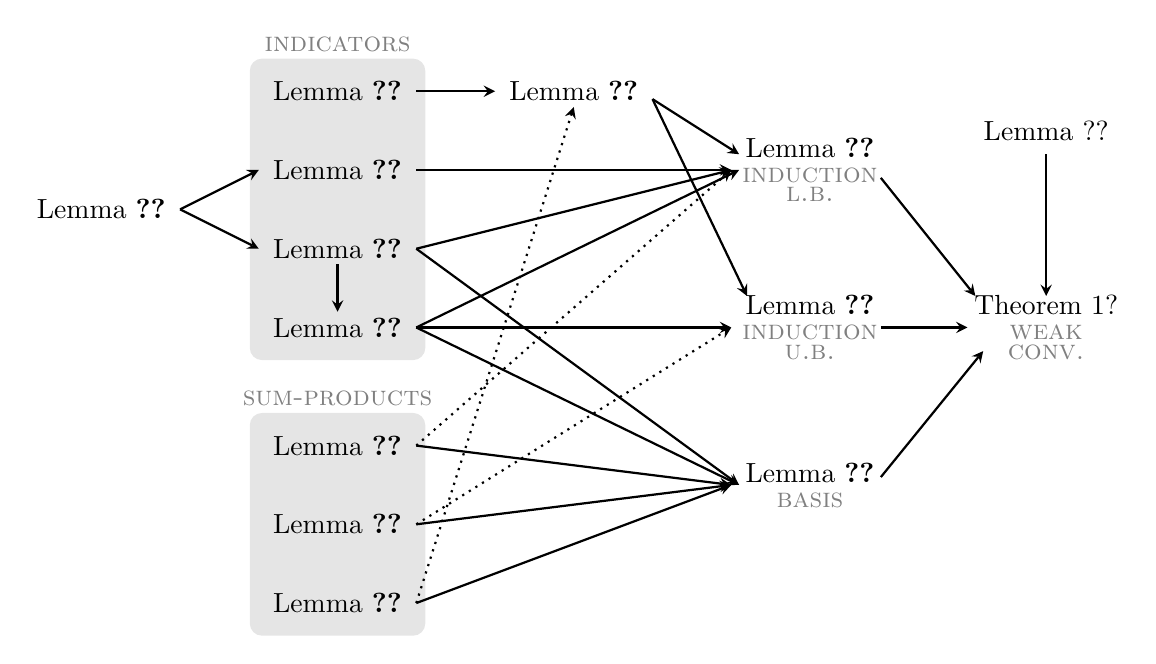
\begin{tikzpicture}[>=stealth, thick]
% boxes
\filldraw[rounded corners, gray!20] (1.9,1.4)--(4.1,1.4)--(4.1,-2.4)--(1.9,-2.4)--cycle;
\node[gray] at (3,1.6) {\textsc{indicators}};
\filldraw[rounded corners, gray!20] (1.9,-3.1)--(4.1,-3.1)--(4.1,-5.9)--(1.9,-5.9)--cycle;
\node[gray] at (3,-2.9) {\textsc{sum-products}};
% nodes column 1
\node at (0,-0.5) {Lemma~\ref{thm:kjjslemma2}};
%nodes column 2 indics
\node at (3,1) {Lemma~\ref{thm:indicators_c2}};
\node at (3,0) {Lemma~\ref{thm:indicators_DN}};
\node at (3,-1) {Lemma~\ref{thm:indicators_cN}};
\node at (3,-2) {Lemma~\ref{thm:indicators_tau}};
% nodes column 2 sumprods
\node at (3,-3.5) {Lemma~\ref{thm:sumprod3}};
\node at (3,-4.5) {Lemma~\ref{thm:sumprod2}};
\node at (3,-5.5) {Lemma~\ref{thm:sumprod1}};
%nodes column 3
\node at (6,1) {Lemma~\ref{thm:induction_sumprodcN}};
% nodes column 4
\node[align=center] at (9,0) {Lemma~\ref{thm:inductionLB}\\[-3pt] \textcolor{gray}{\textsc{induction}} \\[-5pt] \textcolor{gray}{\textsc{l.b.}} };
\node[align=center] at (9,-2) {Lemma~\ref{thm:inductionUB}\\[-3pt] \textcolor{gray}{\textsc{induction}} \\[-5pt] \textcolor{gray}{\textsc{u.b.}} };
\node[align=center] at (9,-4) {Lemma~\ref{thm:basis}\\[-3pt] \textcolor{gray}{\textsc{basis}} };
%nodes column 5
\node at (12,0.5) {Lemma ??};
\node[align=center] at (12,-2) {Theorem 1?\\[-3pt] \textcolor{gray}{\textsc{weak}}\\[-5pt] \textcolor{gray}{\textsc{conv.}} };

% arrows column 1 to 2
\draw[->] (1,-0.5)--(2,0);
\draw[->] (1,-0.5)--(2,-1);
%arrows column 2 to 2
\draw[->] (3,-1.2)--(3,-1.8);
%arrows column 2 to 3
\draw[->] (4,1)--(5,1);
\draw[->, dotted] (4,-5.5)--(6,0.8);
%arrows column2 indics to 4
\draw[->] (4,-2)--(8.1,0);
\draw[->] (4,-2)--(8,-2);
\draw[->] (4,-2)--(8.1,-4);
\draw[->] (4,-1)--(8,0);
\draw[->] (4,-1)--(8.1,-4);
\draw[->] (4,0)--(8,0);
% arrows column 2 sumprods to 4
\draw[->, dotted] (4,-3.5)--(8,0);
\draw[->, dotted] (4,-4.5)--(8,-2);
\draw[->] (4,-3.5)--(8,-4);
\draw[->] (4,-4.5)--(8,-4);
\draw[->] (4,-5.5)--(8,-4);
% arrows column 3 to 4
\draw[->] (7,0.9)--(8.1,0.2);
\draw[->] (7,0.9)--(8.2,-1.6);
%arrows column 4 to 5
\draw[->] (9.9,-0.1)--(11.1,-1.6);
\draw[->] (9.9,-2)--(11,-2);
\draw[->] (9.9,-3.9)--(11.2,-2.3);
% arrows column 5 to 5
\draw[->] (12,0.2)--(12,-1.6);
\end{tikzpicture}
\caption{Graph showing dependencies between lemmata used to prove weak convergence. Dotted arrows indicate dependence via a slight modification.}
\end{figure}

\bibliography{../smc.bib}
\end{document}